\chapter{关系规范化}

\begin{introduction}[期末考试提纲]
  \item 数据异常包括哪些?
  \item 函数依赖、部分函数依赖、完全函数依赖、传递函数依赖、多值依赖
  \item 理解1NF、2NF、3NF、BCNF、4NF的概念
  \item 逻辑蕴含、Armstrong公理
  \item 属性集闭包及其计算, 候选码计算, 范式判定
  \item 函数依赖集等价性判定算法
  \item 最小覆盖计算过程
  \item 关系模式分解的定义和目标, 函数依赖集向属性集的投影
  \item 什么是无损连接分解
  \item 保持函数依赖分解以及判定方法
  \item 保持函数依赖的3NF分解
  \item 保持无损连接的BCNF分解
\end{introduction}

\section{关系模式的设计问题}

信息在关系模式中的表示完全取决于主码。

\begin{table}[H]
  \centering
  \begin{tabular}{|c|c|c|}
    \hline
    \textbf{职工} & \textbf{级别} & \textbf{工资} \\
    \hline
    赵明 & 4 & 500 \\
    \hline
    钱广 & 5 & 600 \\
    \hline
    孙志 & 6 & 700 \\
    \hline
    李开 & 5 & 600 \\
    \hline
    周祥 & 6 & 700 \\
    \hline
  \end{tabular}
  \caption{职工信息表}
\end{table}


\begin{enumerate}
    \item 信息的不可表示问题。
    \begin{enumerate}
        \item 插入异常:如果没有职工具有8级工资,则8级工资的工资数额就难以插入。
        \item 删除异常:如果仅有职工赵明具有4级工资,删除赵明则会将有关4级工资的工资数额信息也一并删除。
    \end{enumerate}
    \item 信息的冗余问题.
    \begin{enumerate}
        \item 数据冗余:职工很多,工资级别有限,每一级别的工资数额反复存储多次。
        \item 更新异常:如果将5级工资的工资数额调为620,则需要找到每个具有5级工资的职工,逐一修改。
    \end{enumerate}
\end{enumerate}

\ 

\fbox{职工}$\to$\fbox{级别}$\to$\fbox{工资}。\textbf{分解}为:\fbox{职工}$\to$\fbox{级别} + \fbox{级别}$\to$\fbox{工资}。

\section{函数依赖}

\begin{definition}[函数依赖] \label{def:func-dep}
  设$R(U)$是属性集$U$上的关系模式, $X,Y\subseteq U$, $r$是$R(U)$上的任意一个关系, 如果成立:
  \begin{center}
    对$\forall t,s\in r$, 若$t[X]=s[X]$, 则$t[Y]=s[Y]$
  \end{center}
  则称``$X$函数决定$Y$''或者``$Y$函数依赖于$X$'', 记作$X\to Y$. 称$X$为决定因素.
\end{definition}

例如, $sno\to sname$, $(sno, cno)\to grade$.

\begin{definition}[函数依赖的双重否定形式的定义] \label{def:func-dep-2}
  不存在$t,s\in r$, $t[X]=s[X]$, 但$t[Y]\neq s[Y]$.
\end{definition}

\begin{definition}[平凡的函数依赖] \label{def:pingfan-func-dep}
  如果$X\to Y$, $Y\subseteq X$, 则称其为平凡的函数依赖. 否则称为非平凡的函数依赖.
\end{definition}

如, $(sno,sname)\to sname$是平凡的函数依赖.

\textit{一个关系模式有$n$个属性,在它上面成立的所有可能的函数依赖有多少个?非平凡的函数依赖有多少个?}

\textbf{Answer.} 需要计算$X\to Y$的个数. 其中$X$和$Y$都是非空子集, 这就可以知道答案为$(2^n-1)^2$.  先计算出平凡的函数依赖个数. 也就是$Y\subseteq X$的个数, $\sum_{k=1}^{n} \binom{n}{k} (2^k-1)=3^n-2^n$. 接着减去这个数, 得到: $2^{2n}-2^n-3^n+1$.


\begin{definition}[完全函数依赖] \label{def:tot-func-dep}
  如果$X\to Y$, 且对于任意$X$的真子集$X'$, 都有$X' \nrightarrow Y$, 则称$Y$对$X$完全函数依赖, 记作$X\overset{f}{\rightarrow} Y$. 否则称$Y$对$X$部分函数依赖, 记作$X\overset{p}{\rightarrow}Y$.
\end{definition}

\begin{definition}[传递函数依赖] \label{def:trans-func-dep}
  在$R(U)$中, 如果: $X\to Y$, $Y\to Z$, $Y\nrightarrow X$, 且$Z\nsubseteq Y$, 则称$Z$对$X$传递函数依赖.
\end{definition}

\begin{remark}
  定义\ref{def:trans-func-dep}中$Y\nrightarrow X$意味着必须通过$Y$来传递, 而$Z\nsubseteq Y$说明并非平凡依赖, 否则可以直接导出$X\to Z$.
\end{remark}

主要问题:如果关系模式设计不当,把本来彼此没有依赖关系的两个属性放在同一个关系模式中,所造成的对候选码的部分依赖和传递依赖是在现实中不存在的,从而会出现异常。
\textit{E.g., 学号$\to$系号, 系号$\to$系主任, 这样学号$\to$系主任, 这是不合理的.}

\section{码的定义(使用函数依赖)}

\begin{definition}[超码]
  设$K$为$R(U,F)$的属性或属性组, 若$K\to U$, 则称$K$为$R$的超码.
\end{definition}

\begin{example}
  $R(ABC;\{A\to B,B\to C\})$有多少超码?

  超码: $\{A,AB,AC,ABC\}$.
\end{example}

\begin{definition}[候选码]
  设$K$为$R(U,F)$的超码, 若$K\overset{f}{\rightarrow} U$, 则称$K$为$R$的候选码.
\end{definition}

\begin{example}
  $R(ABC;\{A\to B,B\to C\})$有多少候选码? $\{A\}$.
\end{example}

\begin{definition}[主属性]
  包含在任意候选码中的属性, 称作主属性.
\end{definition}

\begin{example}
  $R(ABC;\{AB\to C,C\to AB\})$, 计算$R$的主属性. 候选码: $\{AB,C\}$, 主属性: $\{A,B,C\}$.
\end{example}

\begin{definition}[全码]
  关系模式$R(U,F)$的码由整个属性集$U$构成.
\end{definition}

\begin{remark}
  一个全码的关系模式\textbf{不}存在非平凡的函数依赖, 否则就会有更小的码.
\end{remark}

\section{范式}

接下来考虑这个关系模式: $S(\underline{sno},sname,dno,dean,\underline{cno},grade)$.

函数依赖为:
\begin{align*}
  (sno,cno)&\overset{f}{\rightarrow} grade \\
  sno &\to sname \\
  sno &\to dno \\
  dno &\to dean
\end{align*}

数据在表\ref{tab:xuesheng1}中.

\begin{table}[H]
  \centering
  \begin{tabular}{|c|c|c|c|c|c|}
    \hline
    \underline{sno} & sname & dno & dean & \underline{cno} & grade \\
    \hline
    S01 & 杨明 & D01 & 思齐 & C01 & 90 \\ \hline
    S02 & 李婉 & D01 & 思齐 & C01 & 87 \\ \hline
    S01 & 杨明 & D01 & 思齐 & C02 & 92 \\ \hline
    S03 & 刘海 & D02 & 述圣 & C01 & 95 \\ \hline
    S04 & 安然 & D02 & 述圣 & C02 & 78 \\ \hline
    S05 & 乐天 & D03 & 省身 & C01 & 82 \\ \hline
  \end{tabular}
  \caption{学生数据表}
  \label{tab:xuesheng1}
\end{table}

\begin{definition}[范式]
  范式是对关系的不同数据依赖程度的要求.
\end{definition}

\begin{definition}[规范化]
  通过模式分解将一个低级范式转换为若干个高级范式的过程称作规范化.
\end{definition}

\begin{figure}[H]
    \centering
    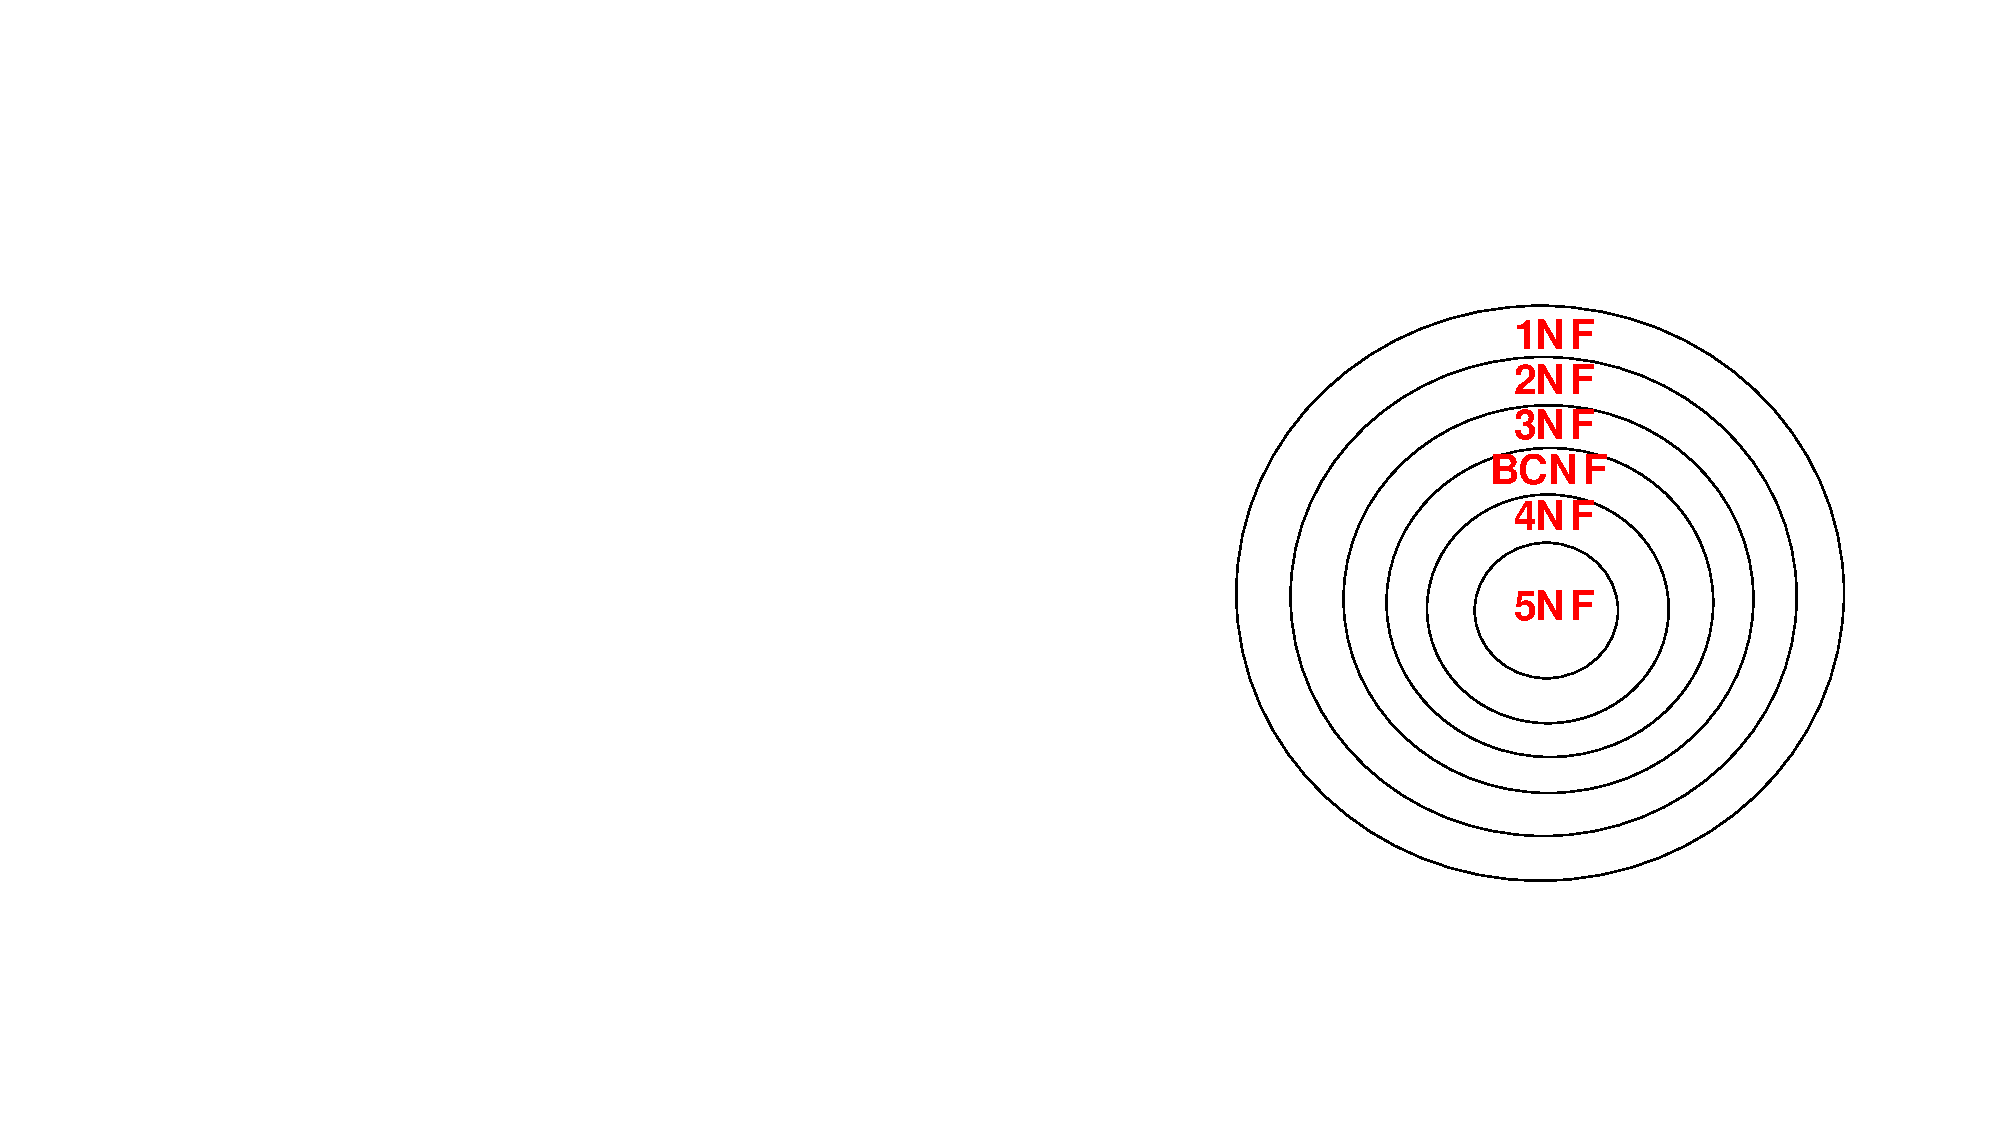
\includegraphics[width=.25\textwidth]{./figure/范式.pdf}
    \caption{范式}
\end{figure}

\subsection{1NF}

\begin{definition}[1NF]
  关系中每一分量\fbox{不可再分}. 也即不能以集合、序列等作为属性值.
\end{definition}

\begin{remark}
  1NF与应用对属性粒度的处理需求有关.

  较细的原子粒度有助于标准化,施加约束避免输入错误,从而提高数据质量。
\end{remark}

\textbf{1NF关系模式的不良特性}, 我们考察表\ref{tab:xuesheng1}.
\begin{enumerate}
    \item 插入异常:如果学生没有选课,关于他的个人信息及所在系的信息就无法插入。
    \item 删除异常:如果删除学生的选课信息,则他的个人信息及所在系的信息也随之删除。
    \item 更新异常:如果学生转系,若他选修了$k$门课,则需要修改$k$次。
    \item 数据冗余:如果一个学生选修了$k$门课,则有关他的所在系的信息重复$k$次。
\end{enumerate}
这些不良特性意味着非主属性对码存在着部分依赖: $(sno,cno)\overset{p}{\rightarrow} sname$, $(sno,cno)\overset{p}{\rightarrow} dno$, $(sno,cno)\overset{p}{\rightarrow} dean$.

从而我们提出了2NF来消除非主属性对码的部分依赖。

\subsection{2NF}

\begin{definition}[2NF]
  若$R\in 1\text{NF}$, 且每个非主属性完全依赖于码, 则称$R\in 2\text{NF}$.
\end{definition}

\begin{remark}
  之前的表\ref{tab:xuesheng1}存在非主属性对码的部分依赖, 不是2NF.
\end{remark}

\begin{example}
  关系模式$R(A,B,C,D)$, 给出它的一个函数依赖集, 使得码为$AB$, 并且$R$属于1NF而不属于2NF.

  $\{AB\to C, A\to D\}$.
\end{example}

如何把关系模式改进到2NF? 把非主属性划分为两部分, 一种是完全依赖于码, 一种是部分依赖于码.

那么我们有: $S_D(\underline{sno},sname,dno,dean)$, $S_C(\underline{sno}, \underline{cno}, grade)$.

但是在关系模式$S_D$中存在着$sno\to dno$, $dno \to dean$, 这就会导致学生和系主任被关联在一起了, 不合理的.

因而我们有3NF: 消除非主属性对码的传递依赖.

\subsection{3NF}

\begin{definition}[3NF]
  关系模式$R(U,F)$中, 若不存在这样的码$X$, 属性组$Y$及非主属性$Z(Z\nsubseteq Y)$, 使得下式成立:
  \begin{align*}
      X\to Y, Y\to Z, Y\nrightarrow X
  \end{align*}
  则称$R\in 3\text{NF}$.
\end{definition}

上面的$S_D \notin 3\text{NF}$.

\begin{example}
  关系模式$R(A,B,C,D)$, 给出它的一个函数依赖集, 使得码为$AB$, 并且R属于2NF而不属于3NF.

  $\{AB\to C, C\to D\}$.
\end{example}

如何将关系改进到3NF? 砸断函数依赖的传递链. $R(ABC,\{A\to B,B\to C\})$分解为$R_1(AB,\{A\to B\})$和$R_2(BC,\{B\to C\})$.

\begin{remark}
  一个全是主属性的关系模式最高一定可以达到3NF. 3NF的目的是为了消除非主属性的冗余.
\end{remark}

3NF的问题: 主属性对码的不良依赖.

\begin{example}
  考虑$STC(sno,tno,cno)$, 我们有:
  \begin{enumerate}
      \item 每位老师只教授一门课: $tno \to cno$.
      \item 某学生选定一门课,就对应一位老师: $(sno,cno)\to tno$.
  \end{enumerate}

  从而候选码为: $(sno, tno)$或$(sno,cno)$. 
  
  一旦没有同学选修, 无法保存一个老师的授课信息.
\end{example}

所以我们考虑BCNF: 所有属性都由码直接决定.

\subsection{BCNF}

\begin{definition}[BCNF]
  关系模式$R(U,F)$中, 对于属性组$X,Y$, 若$X\to Y(Y\nsubseteq X)$,那么$X$必是码, 则$R\in\text{BCNF}$.
\end{definition}

BCNF:所有属性都由码直接决定.

$STC\notin \text{BCNF}$, 因为$tno\to cno$, 但是$tno$不是码.

如何将关系模式改造成BCNF的? 将属性划归到以决定它的属性作为码的关系模式中.

\begin{figure}[H]
    \centering
    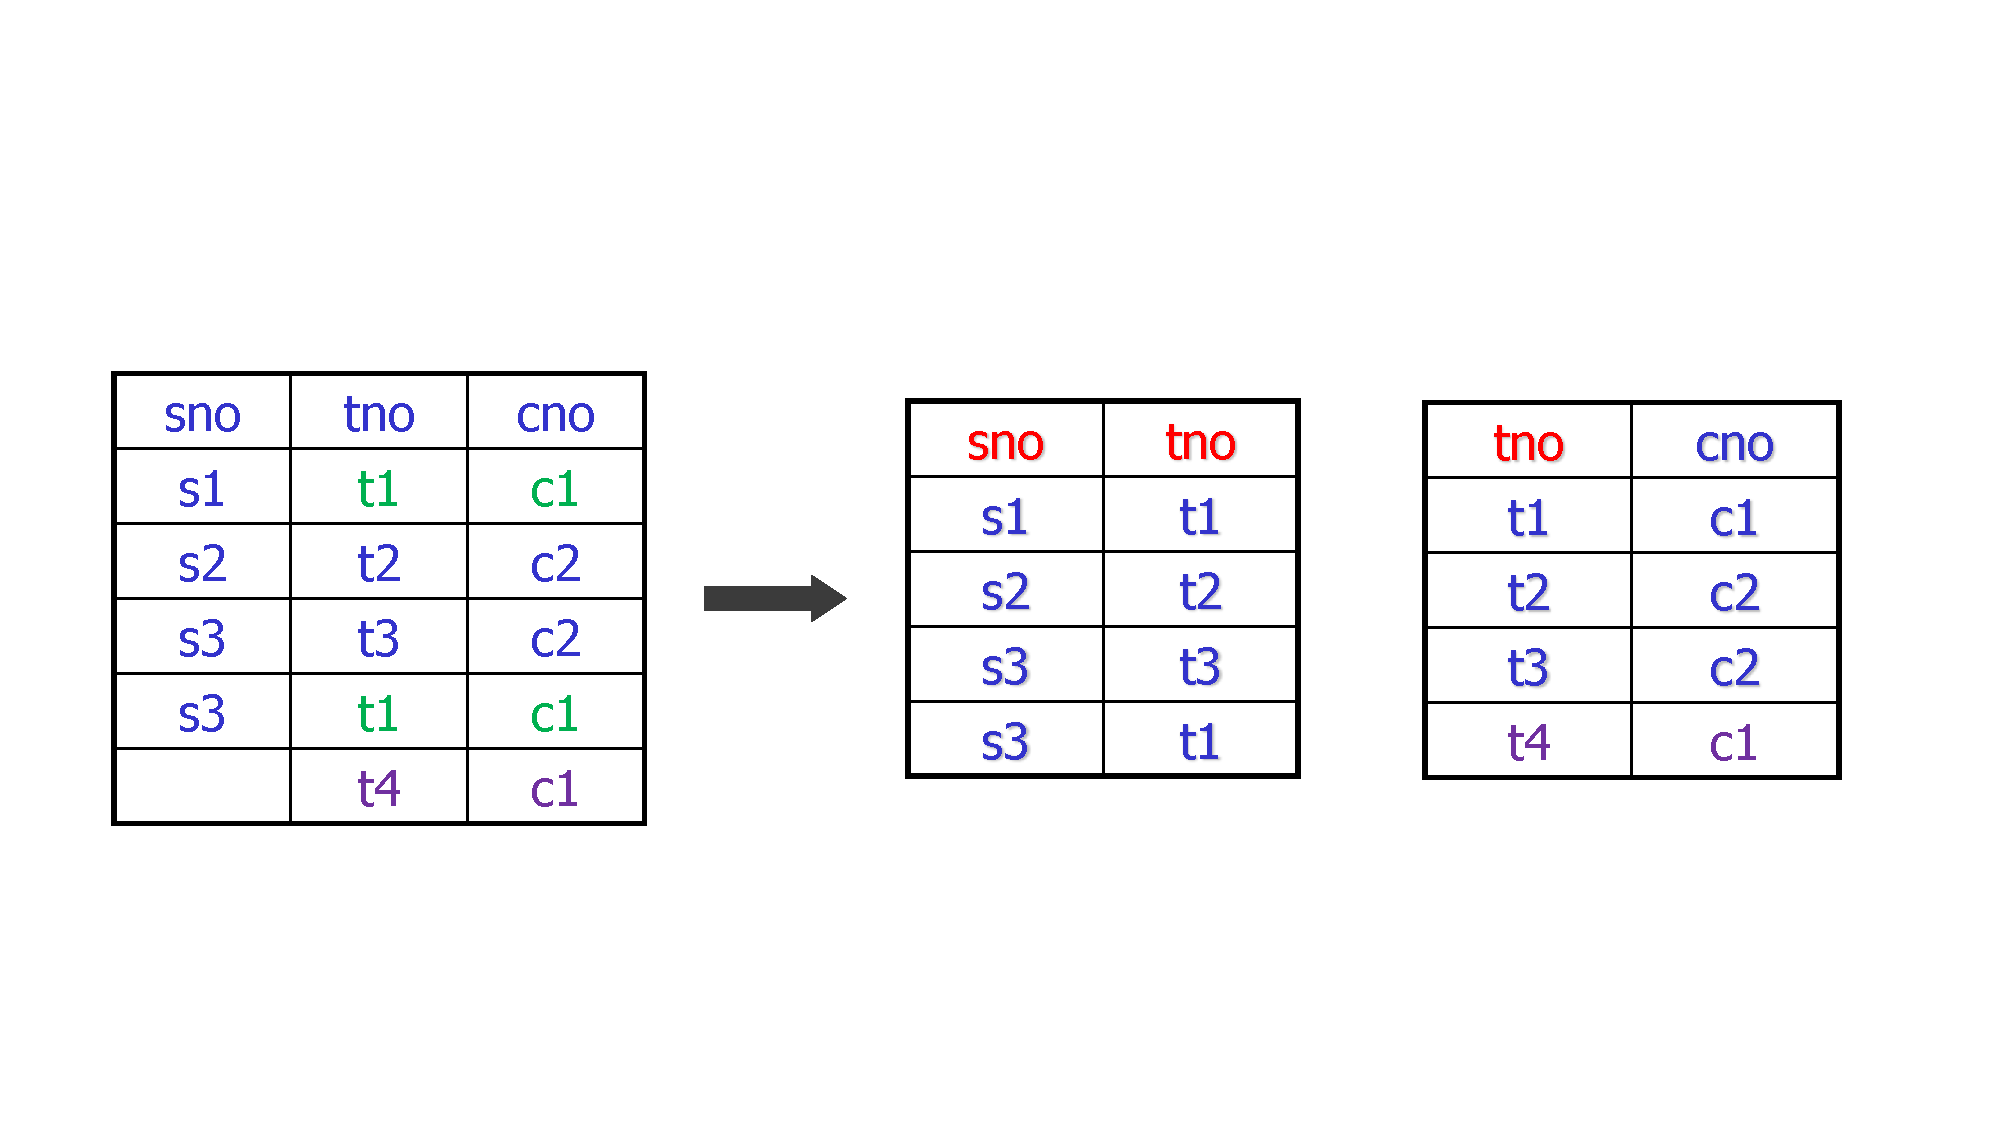
\includegraphics[width=.6\textwidth]{./figure/BCNF.pdf}
    \caption{把关系模式改造为BCNF}
\end{figure}


\begin{example}
  设$(sno,cno,order)$表示学生选课的名次, 假设存在函数依赖$(sno,cno)\to order$, $(cno,order)\to sno$, 请问它属于BCNF吗?

  首先不存在对码的传递依赖和部份依赖, 是3NF. 同时非平凡依赖左边一定是码也是对的. 所以是BCNF.
\end{example}

\begin{definition}[3NF]
  关系模式$R$中的函数依赖$X\to Y$, 满足下述条件之一:
  \begin{itemize}
    \item $X\to Y$是平凡的函数依赖.
    \item $X$是$R$的码.
    \item $Y$是主属性.
  \end{itemize}
\end{definition}

3NF vs. BCNF\quad
存储成本与性能的平衡: 现代存储成本较低, 冗余带来的空间问题可能不如查询性能重要.

\subsection{多值依赖}

\begin{definition}[多值依赖的描述型定义]
  对于关系模式$R(U)$, $X,Y,Z\subseteq U$, $Z=U-X-Y$. 多值依赖$X\to\to Y$成立当且仅当:
  对$R(U)$的任一关系$r$, 给定一对$(x,z)$值对应有一组$Y$的值, 这组$Y$值仅仅决定于$x$值而与$z$值无关. 也就是$\forall x,z, Y_{xz} = Y_x$.
\end{definition}

\begin{figure}[H]
    \centering
    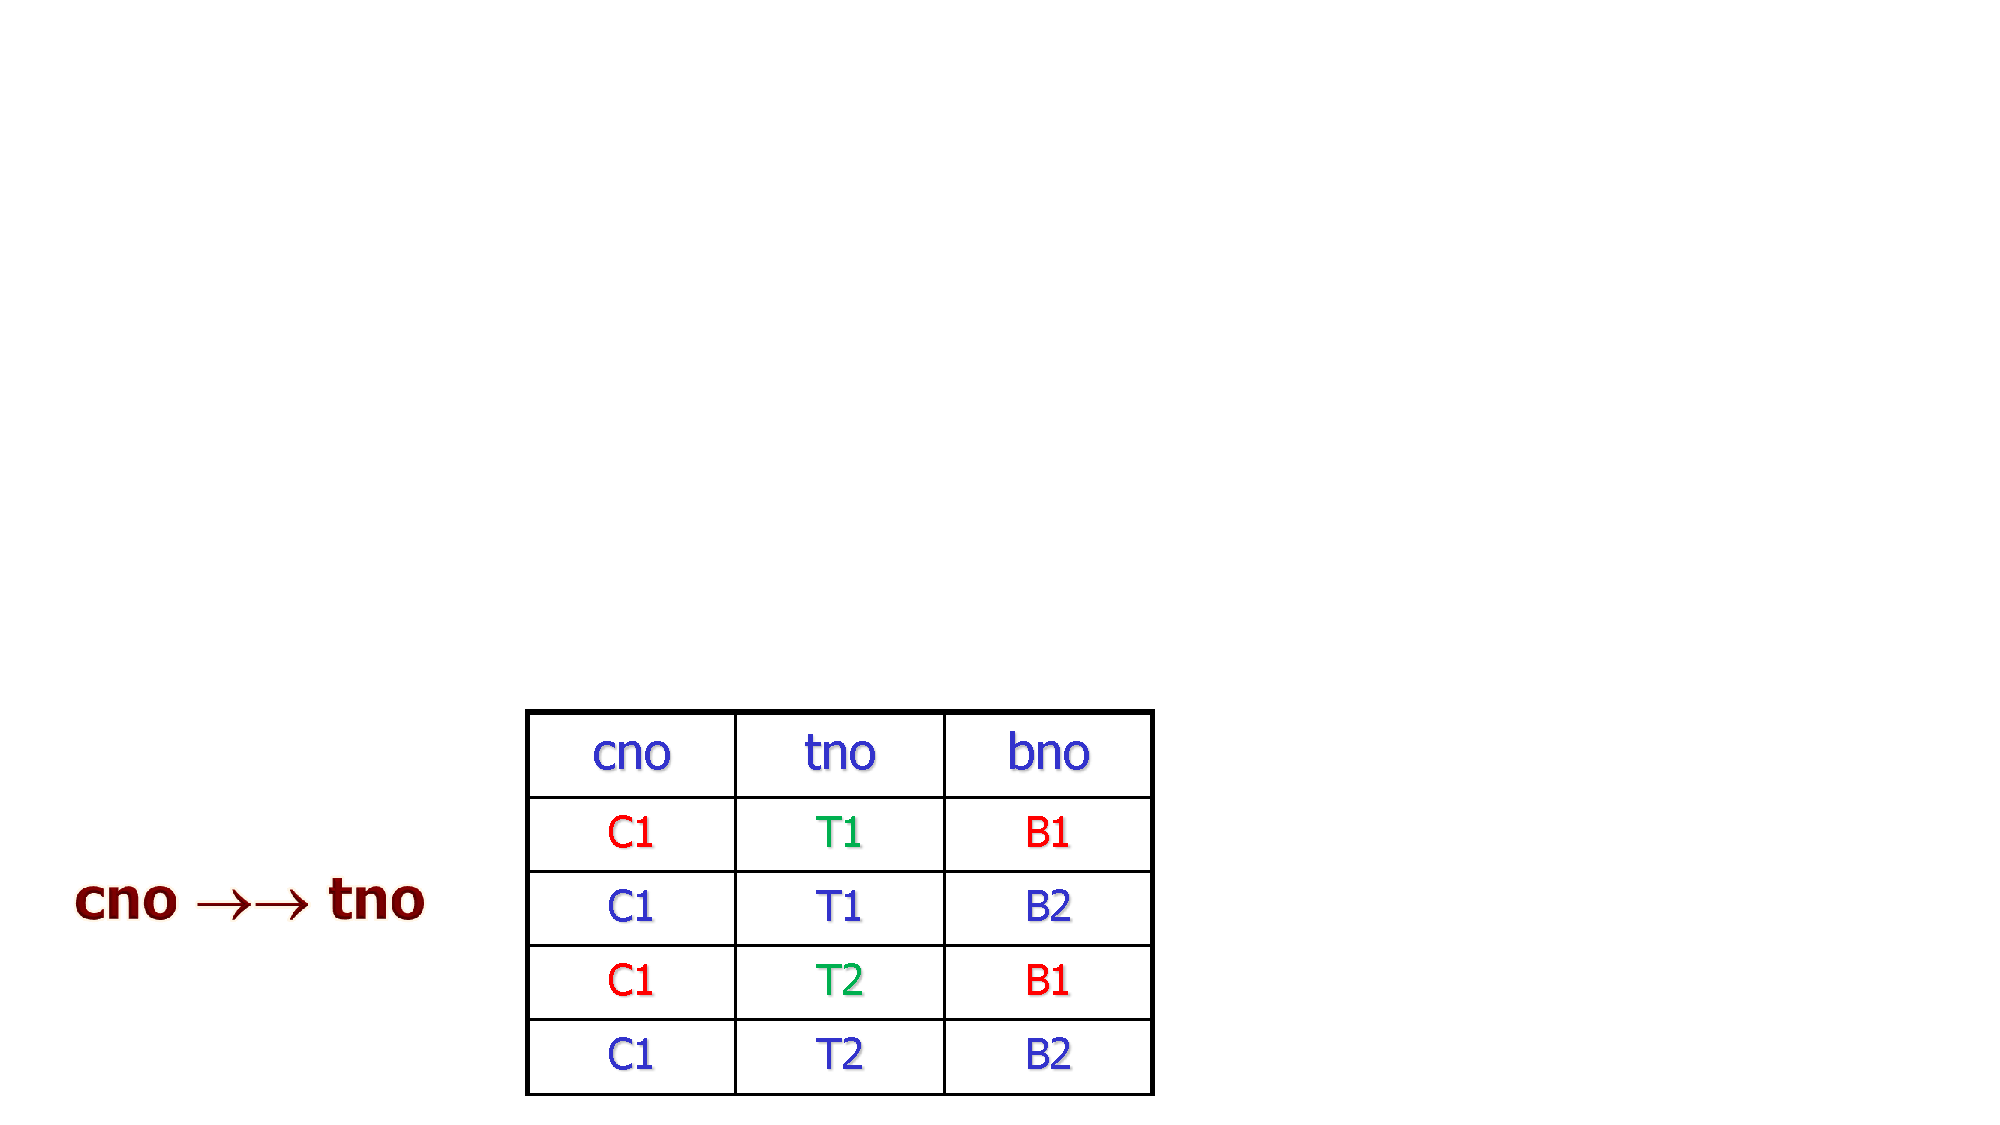
\includegraphics[width=.4\textwidth]{./figure/多值依赖.pdf}
    \caption{多值依赖的例子}
\end{figure}

\begin{definition}[多值依赖的形式化定义]
  关系模式$R(U), X, Y, Z \subseteq U, Z = U - X - Y$.
  对$R(U)$的任一关系$r$, 若存在行$t_1, t_2$, 使得$t_1[X] = t_2[X]$,
  那么就必然存在行 $t_3, t_4$, 使得:
  \begin{align*}
    t_3 &= (t_1[X], t_1[Y], t_2[Z]) \\
    t_4 &= (t_2[X], t_2[Y], t_1[Z]) 
  \end{align*}
  则称$Y$多值依赖于$X$,记作$X \to\to Y$.
\end{definition}

\begin{figure}[H]
    \centering
    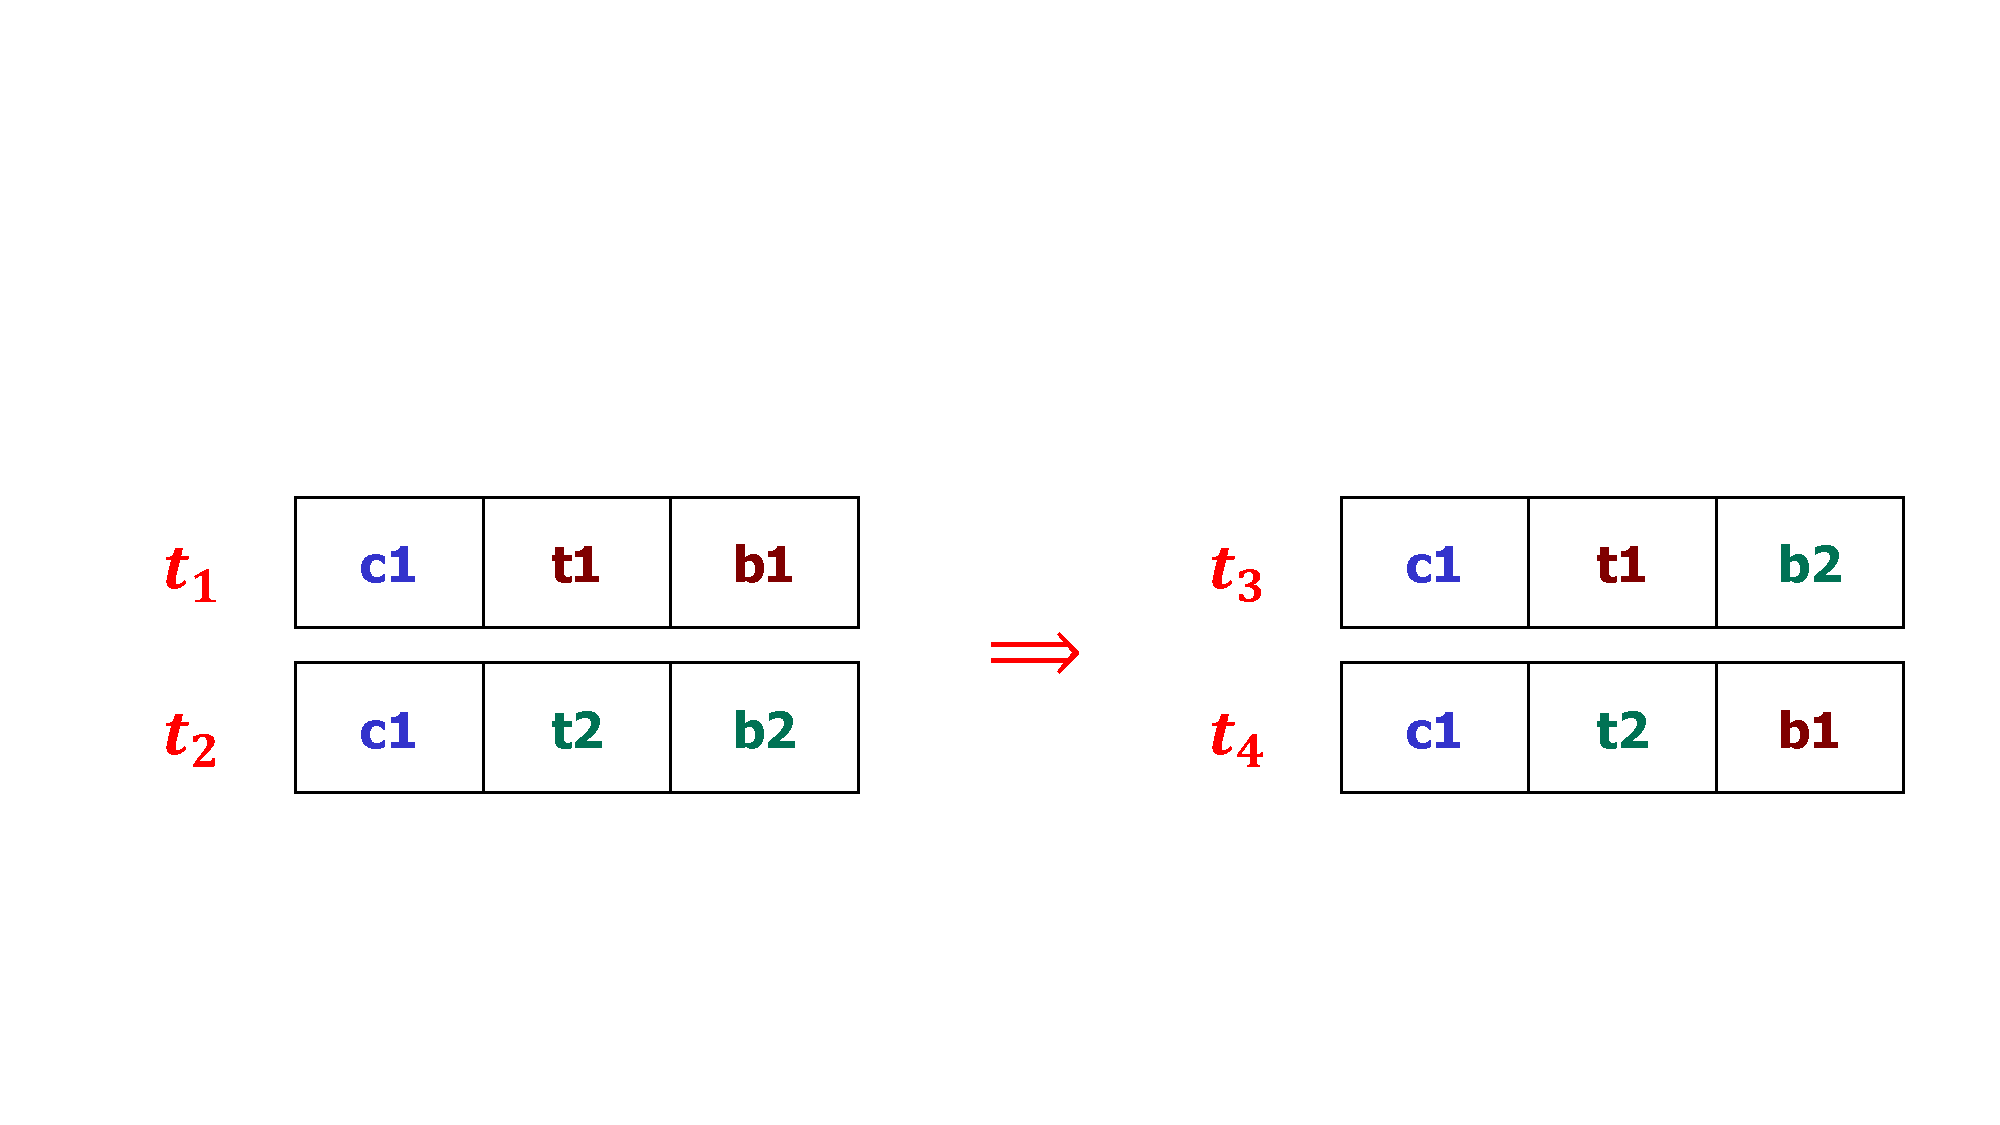
\includegraphics[width=.7\textwidth]{./figure/多值依赖的形式化定义.pdf}
    \caption{多值依赖的形式化定义}
\end{figure}

多值依赖的基本性质:
\begin{enumerate}
    \item 多值依赖具有对称性: 若$X\to\to Y$, 则$X\to\to Z$, 其中$Z=U-X-Y$.
    \item 函数依赖是多值依赖的特例. 若$X\to Y$, 则$X\to\to Y$.
    \item 平凡的多值依赖. 若$X\to\to Y$, $U-X-Y=\varnothing$, 称$X\to\to Y$为平凡的多值依赖.
\end{enumerate}

多值依赖与函数依赖有效性范围的不同:
\begin{itemize}
  \item $X\to Y$的有效性仅决定于$X,Y$属性集上的值. 它在任何属性集$W(XY\subseteq W\subseteq U)$上都成立.
  \item $X\to\to Y$在属性集$W(XY\subseteq W\subseteq U)$上成立, 但在$U$上不一定成立.
\end{itemize}

\begin{definition}[嵌入式多值依赖]
  若 $X \to\to Y$ 在属性集 $W (XY \subseteq W \subseteq U)$ 上成立,
则称 $X \to\to Y$ 为 $R(U)$ 的嵌入式多值依赖.
\end{definition}

\begin{remark}
  $X \to\to Y$ 在 $U$ 上成立 $\Rightarrow$ $X \to\to Y$ 在属性集 $W (XY \subseteq W \subseteq U)$ 上成立. \textbf{这是全集!} $A \to\to B$ 在 $ABCD$ 上成立,则在 $ABC$ 上也成立.

  若 $X \to\to Y$ 在 $R(U)$ 上成立,
  则对于 $\forall Y' \subseteq Y$, 不能确定 $X \to\to Y'$ 是否成立.
  $A \to\to BC$ 成立, $A \to\to B$ 未必成立.
\end{remark}


多值依赖可以保证无损连接: $A\to\to B,A\to\to C \Leftrightarrow r = \Pi_{AB}(r) \bowtie \Pi_{AC}(r)$.

\begin{theorem}[多值依赖成立]
  $A\to\to B$成立当且仅当$R = \Pi_{AB}(R) \bowtie \Pi_{AC}(R)$.
\end{theorem}

\subsection{4NF}

\begin{definition}[4NF]
  关系模式$R(U)\in \text{1NF}$, 对于非平凡的多值依赖$X\to\to Y (Y\nsubseteq X)$, $X$含有码, 则称$R\in\text{4NF}$.
\end{definition}

非4NF的主要弊端: 冗余大. 如果一门课$c_i$有$m$个教员, $n$本参考书, 则$c_i$在关系中一共有$mn$行.

如何将关系模式改造为4NF的? 多值属性单独放在独立的关系模式中.

\subsection{PJNF}

\begin{definition}[连接依赖]
  $R_1(U_1), R_2(U_2), \dots, R_n(U_n)$ 是 $R(U)$ 的一个分解,
  $r$ 是 $R(U)$ 上的一个关系,若 $r = \bowtie_{i=1}^{n} \Pi_{R_i}(r)$,
  则称 $r$ 满足连接依赖 $\leftindex^*(R_1, R_2, \dots, R_n)$.
\end{definition}


连接依赖 $\leftindex^{*}(R_1, R_2, \ldots, R_n)$中, 若有某个 $R_i$ 等于 $R$, 则称之为平凡的连接依赖.

连接依赖 $^{*}(R_1, R_2)$ 等价于多值依赖 $R_1 \cap R_2 \to\to R_1$,
$\alpha \to\to \beta \Leftrightarrow \leftindex^{*}(\alpha \cup (R - \beta), \alpha \cup \beta)$.

\begin{definition}[PJNF]
  若 $R \in \text{PJNF}$, 则对于 $R$ 的任一连接依赖 $\leftindex^{*}(R_1, R_2, \dots, R_n)$ 必是下述情况之一:
  \begin{enumerate}
      \item $\leftindex^{*}(R_1, R_2, \dots, R_n)$ 是平凡的连接依赖
      \item 每个 $R_i$ 是 $R$ 的超码
  \end{enumerate}
\end{definition}

\section{Armstrong公理系统}

\begin{definition}[逻辑蕴含]
  关系模式 $R(U, F)$, $F$ 是其函数依赖集, $X, Y \subseteq U$.
  如果从 $F$ 的函数依赖能够推出 $X \rightarrow Y$,
  则称 $F$ 逻辑蕴涵 $X \rightarrow Y$, 记作 $F \vdash X \rightarrow Y$.
\end{definition}

\begin{definition}[闭包]
  被 $F$ 所逻辑蕴涵的函数依赖的全体所构成的集合称作 $F$ 的闭包, 
  记作 $F^+ = \{X \rightarrow Y \mid F \vdash X \rightarrow Y\}$.
\end{definition}

\begin{theorem}[Armstrong公理系统]
  \begin{itemize}
    \item 自反律(reflexivity): 若 $Y \subseteq X$, 则 $X \rightarrow Y$.
    \item 增广律(augmentation): 若 $X \rightarrow Y$, 则 $XZ \rightarrow YZ$.
    \item 传递律(transitivity): 若 $X \rightarrow Y, Y \rightarrow Z$, 则 $X \rightarrow Z$.
  \end{itemize}
\end{theorem}

\begin{theorem}[正确性]
  设$A=\{f|\text{用Armstrong公理系统从}F\text{中导出的函数依赖}f\}$, 
  
  $B=\{f|\text{被}F\text{所逻辑蕴含的函数依赖}f\}$. 那么正确性就是: $A\subseteq B$.
\end{theorem}

\begin{proof}
  设$r$是$R(U,F)$上的任一关系, $t,s\in r$.
  \begin{enumerate}
      \item 检查自反律. 现在我们设$t[X]=s[X]$, 由于$Y\subseteq X$, 那么$t[Y]=s[Y]$, 那么也就是$X\to Y$. 也就是$X\to Y$可以被$F$(其实$\varnothing$也可以蕴含出)所逻辑蕴含.
      \item 检查增广律. 现在我们设$t[XZ]=s[XZ]$, 那么$t[X]=s[X]$. 结合上$X\to Y$, 那么有$t[Y]=s[Y]$. 同时$t[XZ]=s[XZ]$, 得到$t[Z]=s[Z]$. 最后结合$t[Y]=s[Y]$, $t[Z]=s[Z]$, 得到$t[YZ]=s[YZ]$, 从而得到$XZ\to YZ$.
      \item 检查传递律. 现在我们设$t[X]=s[X]$, 由于$X\to Y$, 得到$t[Y]=s[Y]$. 由于$Y\to Z$, 得到$t[Z]=s[Z]$. 这样就得到了$X\to Z$.
  \end{enumerate}
  综上所述, Armstrong公理系统的正确性得证.
\end{proof}

下面是由Armstrong公理系统推导出的推理规则:
\begin{enumerate}
    \item 合并律(union rule): 若$X\to Y$,$X\to Z$, 则$X\to YZ$.
    \item 分解律(decomposition rule): 若$X\to YZ$, 则$X\to Y$, $X\to Z$.\footnote{一个更强的推论: 若$X\to A_1 A_2 \dots A_n$, 则$X\to A_i$.}
    \item 伪传递律(pseudotransitivity rule): 若$X\to Y$, $WY\to Z$, 则$WX\to Z$.
\end{enumerate}

\section{闭包计算}

\begin{definition}[属性集的闭包]
  设$F$为属性集$U$上的一组函数依赖, $X\subseteq U$,
  \begin{align*}
    X_F^+=\{A|X\to A\text{能由}F\text{根据Armstrong公理系统推出}\},
  \end{align*}
  称$X_F^+$为属性集$X$关于函数依赖集$F$的闭包.
\end{definition}

\begin{algorithm}[H]
\caption{属性集 $X$ 关于函数依赖集 $F$ 的闭包 $X_F^+$ 的计算}
\label{algo:bibao}
\KwIn{属性集 $X$,函数依赖集 $F$}
\KwOut{$X_F^+$}

$X_F^+ \gets X$\;

\Repeat{$X_F^+$ 不再发生变化}{
    \ForEach{函数依赖 $A \rightarrow B \in F$}{
        \If{$A \subseteq X_F^+$}{
            $X_F^+ \gets X_F^+ \cup B$\;
        }
    }
}
\end{algorithm}


算法\ref{algo:bibao}的正确性: 
\begin{align*}
  A \subseteq X_F^+ \Rightarrow X\to A, A \to B \Rightarrow X\to B \Rightarrow B \in X_F^+.
\end{align*}

算法最多$|U-X|$步终止(每次都加入一个属性).

\begin{theorem}[闭包的封闭性]
  $(X^+)^+=X^+$.
\end{theorem}
\begin{proof}
  我们设$A\in(X^+)^+$, 那么就有$X^+\to A$, 同时我们有$X\to X^+$, 那么就有$X\to A$.
  那么$A\in X^+$, 这样就导出了$(X^+)^+\subseteq X^+$. 同时原本就有$X^+\subseteq (X^+)^+$, 
  那么$(X^+)^+=X^+$.
\end{proof}

\begin{definition}[属性集的封闭性]
  如果$X^+=X$, 则称$X$是\textcolor{red}{封闭}的.
\end{definition}

如何判断$X\to Y$是否可以由Armstrong公理系统导出?
\begin{enumerate}
    \item 计算出$F^+$, 再判断$X\to Y$是否属于$F^+$. \textit{计算很复杂!}
    \item 判断$Y\subseteq X_F^+$是否成立. \textit{简单. 判断依据来自于下面的定理.}
\end{enumerate}

\begin{theorem}
  $X\to Y$能由Armstrong公理系统导出 $\Leftrightarrow$ $Y\subseteq X_F^+$.
\end{theorem}

同时我们现在也可以借助属性集的闭包来说明Armstrong公理系统的完备性.
\begin{theorem}[完备性]
  设$A=\{f|\text{用Armstrong公理系统从}F\text{中导出的函数依赖}f\}$, 
  
  $B=\{f|\text{被}F\text{所逻辑蕴含的函数依赖}f\}$. 那么正确性就是: $B\subseteq A$.
\end{theorem}

\begin{proof}
  我们使用\textcolor{red}{反证法}.

  若存在函数依赖$X\to Y$被$F$逻辑蕴含, 但$X\to Y$不能用Armstrong公理系统从$F$中导出.
  
  则存在$Y$的子集不属于$X$的闭包, 也即$Y-X_F^+\neq \varnothing$, $U-X_F^+\neq \varnothing$.

  下面我们构造一个$R(U)$上的关系$r$:
  \begin{align*}
    \begin{array}{c|cc}
      \textcolor{red}{r} & \textcolor{blue}{X_F^+} & \textcolor{blue}{U - X_F^+} \\
      \hline
      \textcolor{blue}{t} & 1 & 0 \\
      \textcolor{blue}{s} & 1 & 1 \\
    \end{array}
  \end{align*}
  下面证明和我们的假设互相矛盾的两条结论:
  \begin{enumerate}
      \item $r$满足$F$.

      设$W\to V$是$F$中的任一一个函数依赖. 我们设$t[W]=s[W]$, 那么$W\subseteq X_F^+$, 在另一边不可能会有$t[W]=s[W]$. 这样就得到$X\to W$, 利用传递性得到$X\to V$, 从而$V\subseteq X_F^+$, 从而$t[V]=s[V]$. 所以$r$满足函数依赖$W\to V$, 也即$r$是$R(U,F)$上的关系.
      \item $r$不满足$X\to Y$.

      $Y-X_F^+\neq \varnothing$, 所以存在$A\not\in X_F^+$. 但是有$t[X]=s[X]$, $t[A]\neq s[A]$, 所以$t[Y]\neq s[Y]$, 也即$X\to Y$不成立.
  \end{enumerate}
  那么假设就不成立, 完备性得到证明.
\end{proof}

\section{候选码计算}

\begin{definition}[左部属性]
  \textcolor{red}{左部属性}, 只出现在$F$左边的属性.
\end{definition}

\begin{definition}[右部属性]
  \textcolor{green!60!black}{右部属性}, 只出现在$F$右边的属性.
\end{definition}

\begin{definition}[双部属性]
  \textcolor{violet}{双部属性}, 出现在$F$两边的属性.
\end{definition}

\begin{definition}[外部属性]
  \textcolor{brown}{外部属性}, 不出现在$F$中的属性.
\end{definition}

\begin{enumerate}
    \item \textcolor{red}{左部属性}一定出现在任何候选码中.
    \item \textcolor{green!60!black}{右部属性}一定不出现在任何候选码中.
    \item \textcolor{brown}{外部属性}一定出现在任何候选码中.
\end{enumerate}

候选码的构成: \textcolor{red}{左部属性} + \textcolor{brown}{外部属性} + [可能出现的\textcolor{violet}{双部属性}].

\begin{example}
  设$U=\{C,T,H,R,S\}$, $F=\{C\to T,HR\to C,HT\to R,HS\to R\}$, 给出$R$的所有候选码, 判断其范式级别.
\end{example}

左部属性为$\{H,S\}$, 双部属性为$\{C,T,R\}$. 注意到$(HS)_F^+=HSRCT$, 所以候选码为$HS$.

\begin{algorithm}[H]
    \KwIn{关系模式$R(U, F)$}
    \KwOut{一个候选码$K$}
    
    \caption{寻找一个候选码的一般算法}
    
    $K := U$\;
    构造一个FD: $K \rightarrow T$, 其中 $T \notin U$\;
    
    \For{每一个属性 $A \in K$}{
        \If{Membership$(F \cup \{K \rightarrow T\}, (K-A) \rightarrow T)$}{
            $K := K - A$\; 
            \Comment{$Membership(F,X\to Y)$判断是否有$X\to Y\in F^+$}
        }
    }
    return($K$)\;
\end{algorithm}

\begin{algorithm}[H]
    \KwIn{关系模式$R(U, F)$}
    \KwOut{$R(U,F)$的全部候选码}
    
    \caption{寻找全部候选码的算法}
    
    $K := $找到一个候选码\;
    $K$入队列$Q$\;
    \While{队列 $Q \neq \emptyset$}{
      $K :=$ 队列 $Q$ 的头\;
      $W := W \cup \{K\}$\;
      $D := K$ 中全部双部属性\;
        
      \While{$D \neq \emptyset$}{
        $A := D$ 中一个双部属性\;
        $D := D - \{A\}$\;
            
        \For{每一个 $X \rightarrow Y \in F$}{
          \If{$A \in Y$}{
            $K' := (K - A) \cup \{X\}$\;
            \If{$K' \notin Q$}{
              $K'$ 入队列 $Q$\;
            }
          }
        }
      }
    }
  return($W$)\;
\end{algorithm}

\section{函数依赖的等价和覆盖}

\begin{definition}[函数依赖集的等价性]\label{def:fd-eq}
  对于函数依赖集$F,G$, 若\textcolor{red}{$F^+=G^+$}, 则称\textcolor{red}{$F$与$G$等价}.
\end{definition}

定义\ref{def:fd-eq}实际上要求我们检验: \textcolor{red}{$F\subseteq G^+\land G\subseteq F^+$.}

\begin{definition}[函数依赖集的最小覆盖]
  对于函数依赖集, 它的最小覆盖$F$满足下面的三个条件:
  \begin{enumerate}
      \item \textcolor{red}{单属性化.} 对于$F$中任一函数依赖$X\to A$, $A$必是单属性.
      \item \textcolor{red}{无冗余化.} $F$中不存在这样的函数依赖$X\to A$, 使得$F$与$F-\{X\to A\}$等价.
      \item \textcolor{red}{既约化.} $F$中不存在这样的函数依赖$X\to A$, 在$X$中有真子集$Z$, 使得$F$与$F-\{X\to A\}\cup \{Z\to A\}$等价.
  \end{enumerate}
\end{definition}

下面给出求解函数依赖集$F$的最小覆盖$F_{min}$的算法:
\begin{enumerate}
    \item \textcolor{red}{单属性化:} 逐个检查$F$中各函数依赖$FD_i: X\to Y$, 若$Y=A_1A_2\dots A_k$, 则用诸$X\to A_i$代替$Y$.
    \item \textcolor{red}{无冗余化:} 逐个检查$F$中各函数依赖$X\to A$, 令$G=F-\{X\to A\}$, 若$A\in X_G^+$, 则从$F$中去掉该函数依赖.
    \item \textcolor{red}{既约化:} 逐个检查$F$中各函数依赖$X\to A$, 设$X=B_1B_2\dots B_m$, 逐个考察$B_i$, 若$A\in (X-B_i)_F^+$, 则$X-B_i$取代$X$.
\end{enumerate}

\begin{example}
  已知$F=\{A\to B,B\to A,A\to C,B\to C\}$, 求$F_{min}$.
\end{example}

检查 $A \rightarrow B$, $G = F - \{A \rightarrow B\} = \{B \rightarrow A, A \rightarrow C, B \rightarrow C\}$

$ A_G^+ = \{A, C\} \Rightarrow B \notin A_G^+ \Rightarrow A \rightarrow B \notin G^+ $.

检查 $A \rightarrow C$, $G = F - \{A \rightarrow C\} = \{A \rightarrow B, B \rightarrow A, B \rightarrow C\}$

$ A_G^+ = \{A, B, C\} \Rightarrow C \in A_G^+ \Rightarrow A \rightarrow C \in G^+ $.

$ F_{min} = \{A \rightarrow B, B \rightarrow A, B \rightarrow C\} \quad \text{或者} \quad F_{min} = \{A \rightarrow B, B \rightarrow A, A \rightarrow C\} $.


\section{函数依赖和多值依赖的推理规则}

\begin{enumerate}
    \item 自反律: 若$Y\subseteq X$, 则$X\to Y$.
    \item 增广律: 若$X\to Y$, 则$XZ\to YZ$.
    \item 传递律: 若$X\to Y$, $Y\to Z$, 则$X\to Z$.
    \item 复制律: 若$X\to Y$, 则$X\to\to Y$.
    \item 补充律: 若$X\to\to Y$, 则$X\to\to R-X-Y$.
    \item 多值增广律: 若$X\to\to Y$, $Z\subseteq R$, $W\subseteq Z$, 则$XZ\to\to YW$.
    \item 多值传递律: 若$X\to\to Y$, $Y\to\to Z$, 则$X\to\to Z-Y$.
    \item 联合律: 若$X\to\to Y$, $Z\subseteq Y$, 且存在$W$, 使得$W\subseteq R$, $W\cap Y=\varnothing$, $W\to Z$, 则$X\to Z$.
\end{enumerate}

\section{模式分解}

\begin{definition}[函数依赖在属性集上的投影]
  函数依赖集$F$在属性集$U_i$上的投影定义为:
  \begin{align*}
    F_i = \{X\to Y|X\to Y\in F^+ \land XY\subseteq U_i\}.
  \end{align*}
\end{definition}

\begin{remark}
  要判断$X\to Y\in F^+$, 只需要判断$Y\in X_F^+$.
\end{remark}

\begin{example}
  求$F=\{A\to B,B\to C,C\to D\}$在$S(ACD)$上的投影.
\end{example}

首先计算出: $A_F^+=ABCD, C_F^+=CD,D_F^+=D$. 那么从而得到投影为$\{A\to C,A\to D,C\to D\}$.
现在考虑右侧可以组合成的$CD$, $(CD)_F^+=CD$, 从而投影确实为$\{A\to C,A\to D,C\to D\}$.

\begin{example}
  计算下面的函数依赖集在$S(ABC)$上的投影:
  \begin{enumerate}
      \item $F=\{AB\to DE, C\to E, D\to C, E\to A\}$;
      \item $F=\{A\to D,BD\to E, AC\to E, DE\to B\}$;
      \item $F=\{AB\to D, AC\to E,BC\to D,D\to A,E\to B\}$.
  \end{enumerate}
\end{example}


\begin{definition}[模式分解]
  关系模式$R(U,F)$的一个分解是指
  \begin{align*}
    \rho = \{R_1(U_1,F_1), R_2(U_2,F_2),\dots,R_n(U_n,F_n)\},
  \end{align*}
  其中$U=\bigcup_{i=1}^n U_i$, 并且没有$U_i\subseteq U_j$, $1\leq i,j\leq n$, $F_i$是$F$在$U_i$上的投影.
\end{definition}

\subsection{保持函数依赖分解}

\begin{definition}[保持函数依赖分解]
  设关系模式$R(U,F)$的一个分解是
  \begin{align*}
    \rho = \{R_1(U_1,F_1), R_2(U_2,F_2),\dots,R_n(U_n,F_n)\},
  \end{align*}
  如果\textcolor{red}{$F^+=\left(\bigcup_{i=1}^n F_i\right)^+$},
  则称$\rho$是保持函数依赖的分解.
\end{definition}

保持函数依赖 $\Leftrightarrow$ \textcolor{red}{$F^+=\left(\bigcup_{i=1}^n F_i\right)^+$}
$\Leftrightarrow$ \textcolor{red}{$F\subseteq \left(\bigcup_{i=1}^n F_i\right)^+ \land F_i \subseteq F^+$}.


\subsection{保持无损连接分解}

\begin{definition}[无损连接分解]
  关系模式$R(U,F)$, $U=\bigcup_{i=1}^n U_i$, $\rho = \{R_1(U_1,F_1), R_2(U_2,F_2),\dots,R_n(U_n,F_n)\}$, $r$是$R$的任意一个关系实例, 定义
  \begin{align*}
    m_{\rho}(r) = \bowtie_{i=1}^n \Pi_{U_i}(r).
  \end{align*}
  若\textcolor{red}{$m_{\rho}(r)=r$}, 则称$\rho$是$R$的一个无损分解.
\end{definition}

\begin{figure}[H]
    \centering
    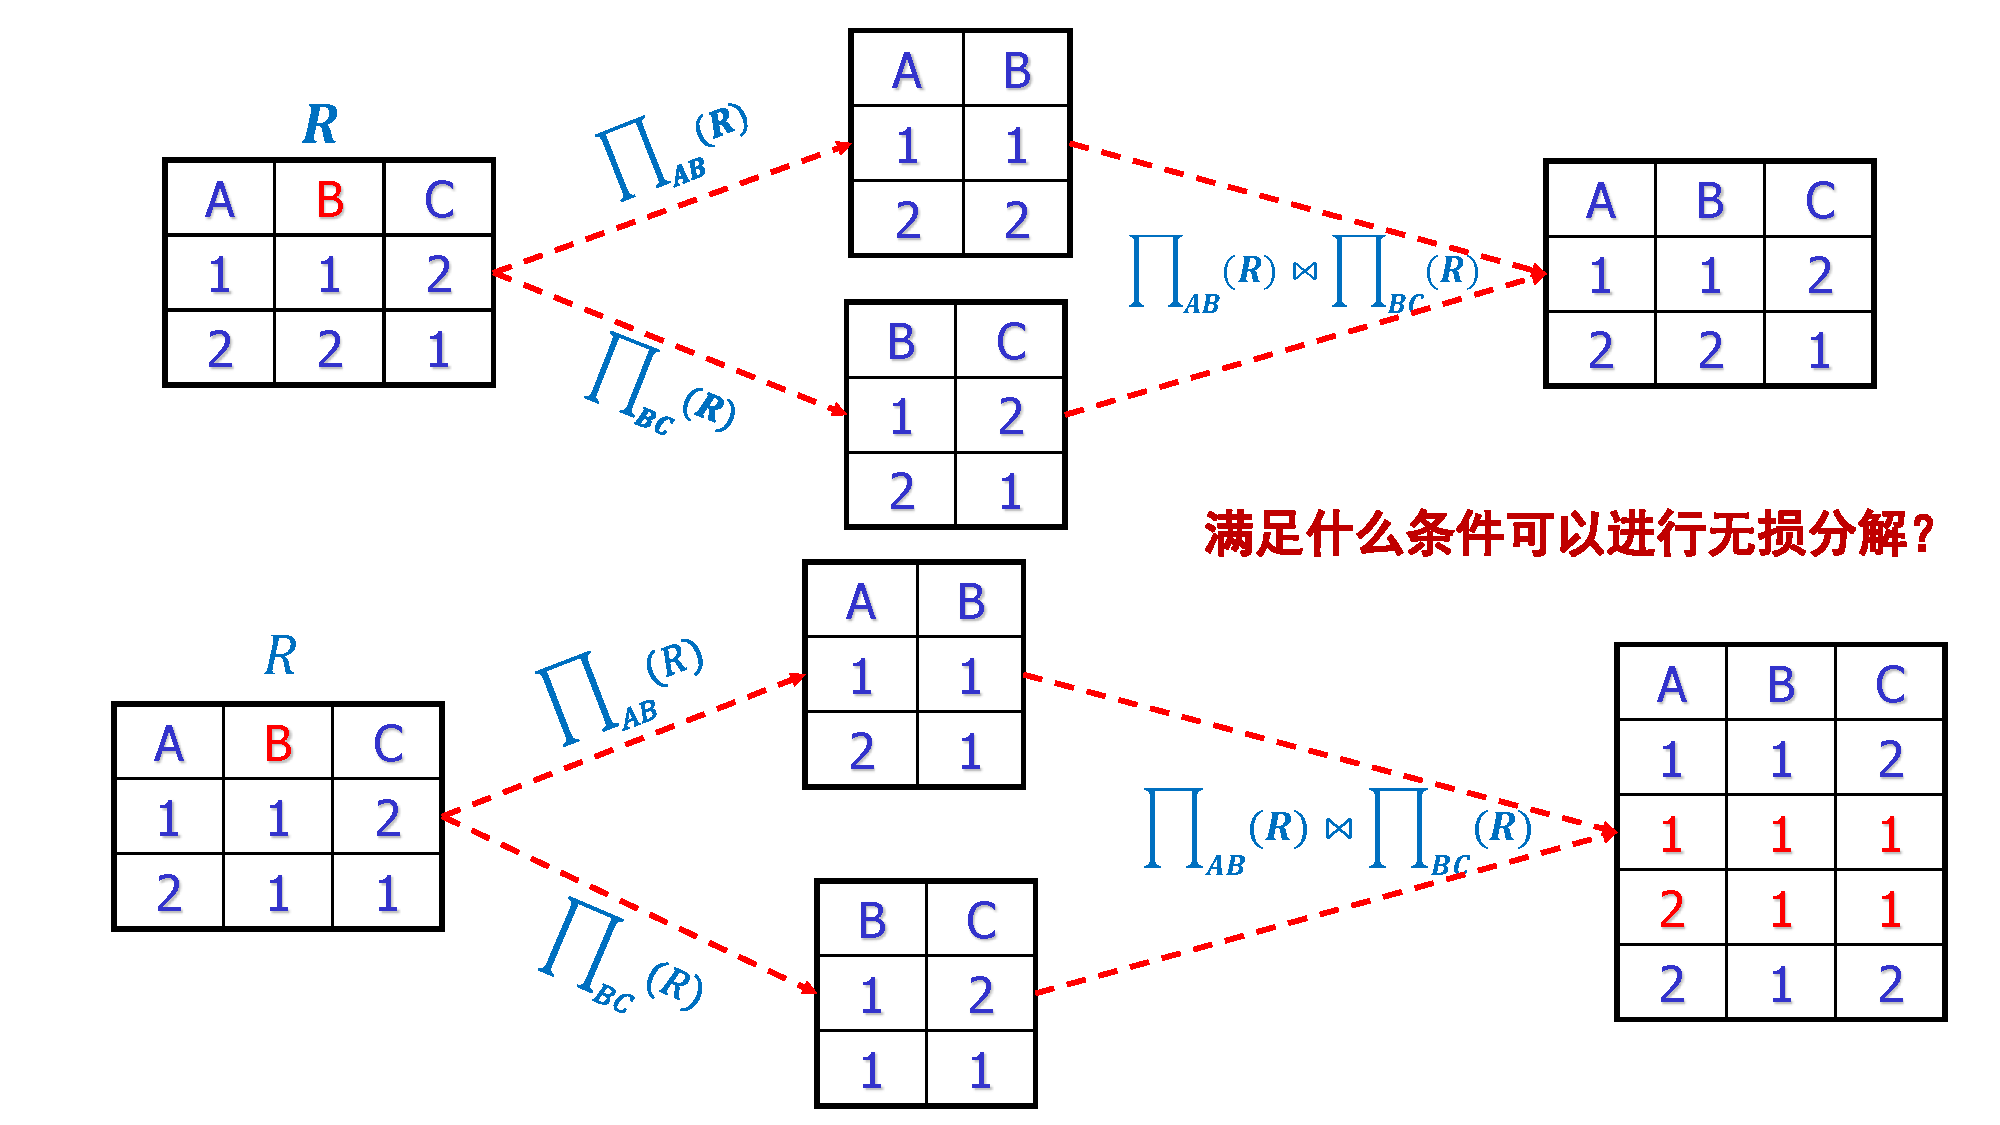
\includegraphics[width=.6\textwidth]{./figure/无损分解.pdf}
    \caption{无损分解的例子}
\end{figure}

\textbf{无损连接分解的判别算法.}

对于$U=\{A_1,A_2,\dots,A_n\}$, $\rho=\{R_1(U_1,F_1),R_2(U_2,F_2),\dots,R_k(U_k,F_k)\}$.
\begin{enumerate}
    \item \textcolor{red}{建立一个$k$行$n$列的矩阵}(行是子模式$U_i$, 列是$U$中属性$A_j$), 其中:
    \begin{align*}
      TB = \{C_{ij} | \text{若}A_j\in U_i, C_{ij}=a_j, \text{否则}C_{ij}=b_{ij}\}.
    \end{align*}
    \item 对$F$中的每一个函数依赖$X\to Y$, 若$TB$中存在元组$t_1,t_2$, 使得\textcolor{red}{$t_1[X]=t_2[X], t_1[Y]\neq t_2[Y]$}. 则对每一个$A_i\in Y$:
    \begin{enumerate}
        \item 若$t_1[A_i],t_2[A_i]$中有一个等于$a_i$, 则另一个也改为$a_j$;
        \item 若(a).不成立, 则取$t_1[A_i]=t_2[A_i]$ ($t_2$的行号小于$t_1$).
    \end{enumerate}
    \item 反复执行2., 直至:
    \begin{enumerate}
        \item $TB$中出现一行全为\textcolor{red}{$a_1,a_2,\dots,a_n$}的一行, 此时$\rho$为\textcolor{red}{无损分解};
        \item $TB$不再发生变化, 且没有一行为$a_1,a_2,\dots,a_n$, 此时$\rho$为\textcolor{red}{有损分解}.
    \end{enumerate}
\end{enumerate}

\begin{example}
  判断下面的分解是否是无损分解.
  
  $U=\{A,B,C,D,E\},F=\{AB\to C,C\to D,D\to E\}$, $\rho = \{ABC,CD,DE\}$.
\end{example}

\begin{figure}[H]
    \centering
    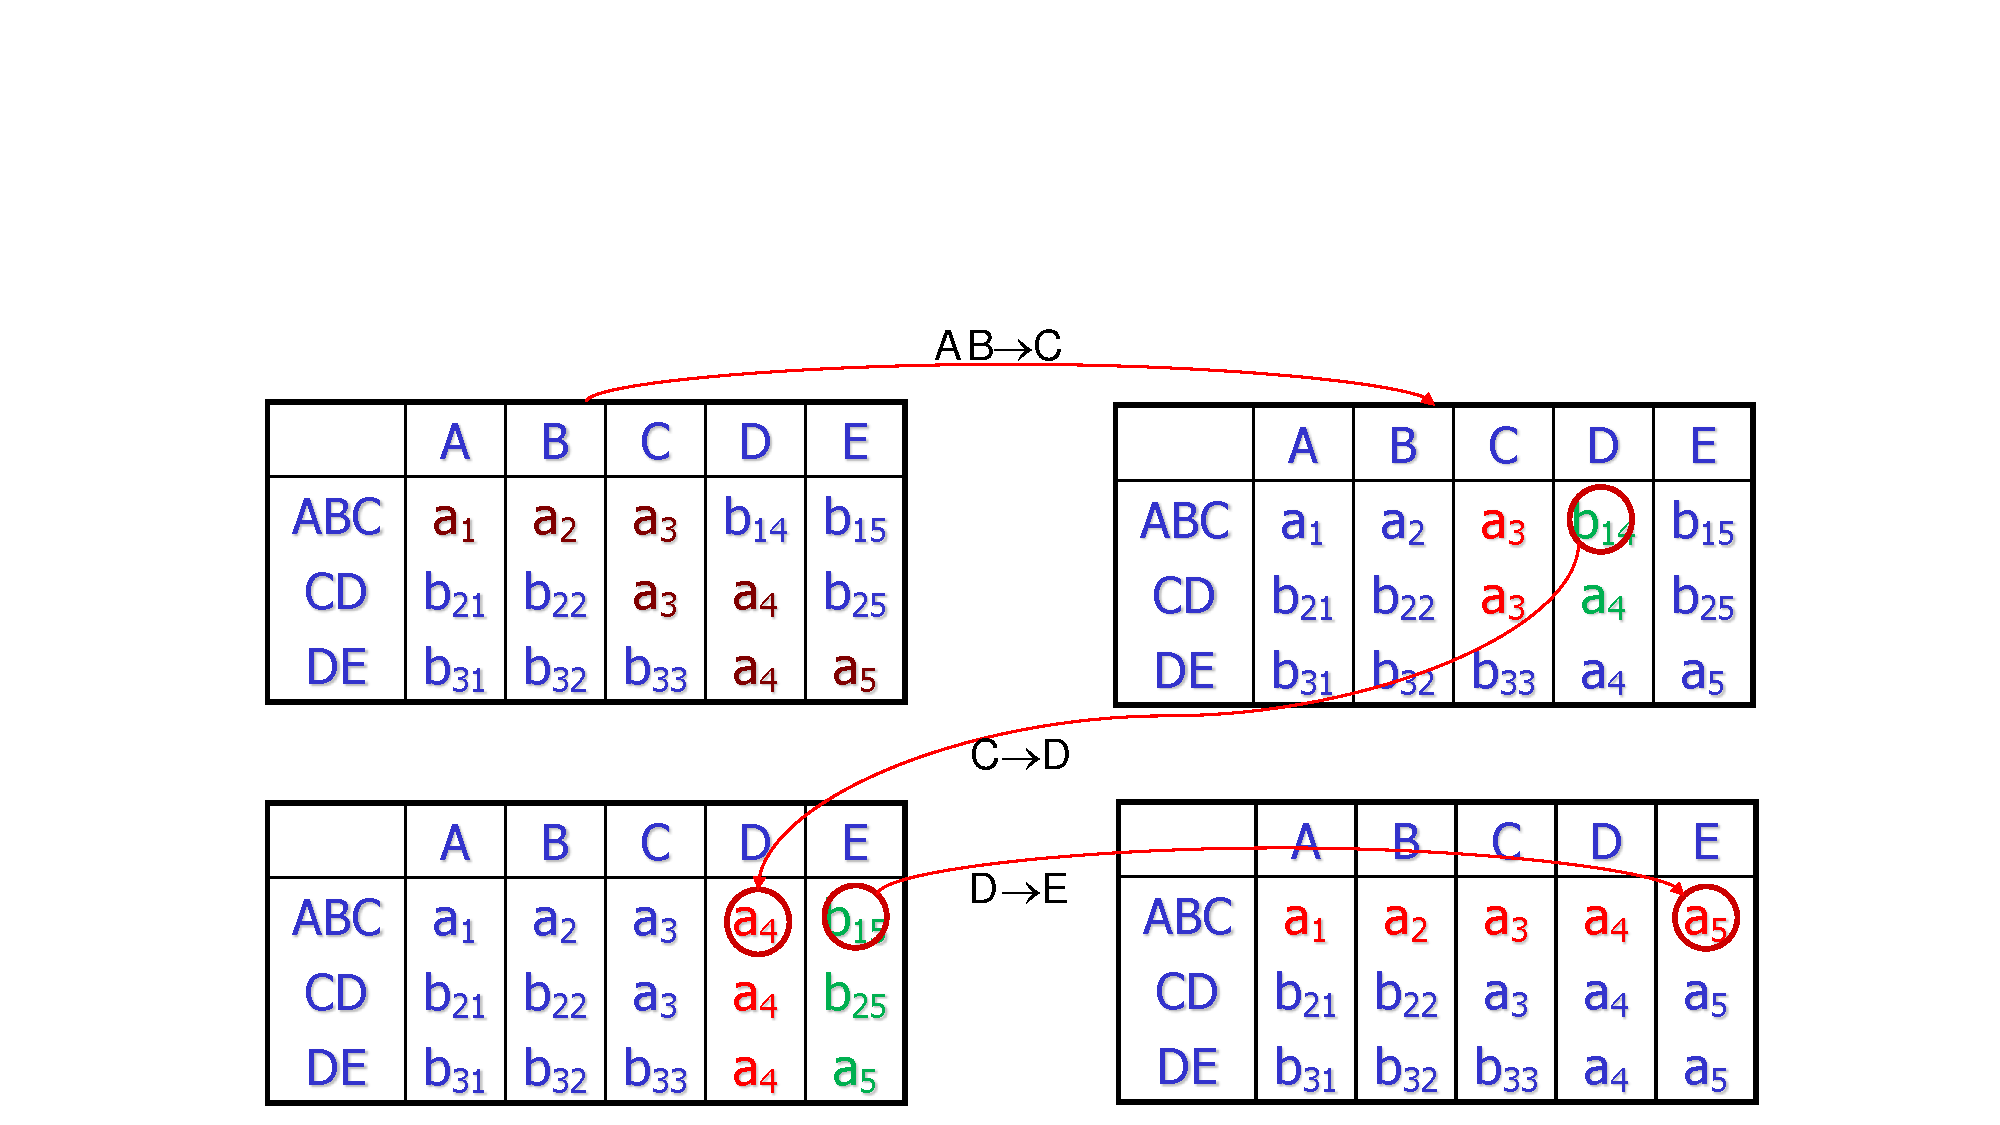
\includegraphics[width=.5\textwidth]{./figure/无损分解判定.pdf}
    \caption{无损连接分解判别算法示例}
\end{figure}

\begin{example}
  判断下面的分解是否是无损分解.
  
  $U=\{ A, B, C, D, E \},F = \{ A \rightarrow C, B \rightarrow C, C \rightarrow D, DE \rightarrow C, CE \rightarrow A \}$,  
  
  $\rho = \{ AD, AB, BE, CDE,AE\}$.
\end{example}

\begin{figure}[H]
    \centering
    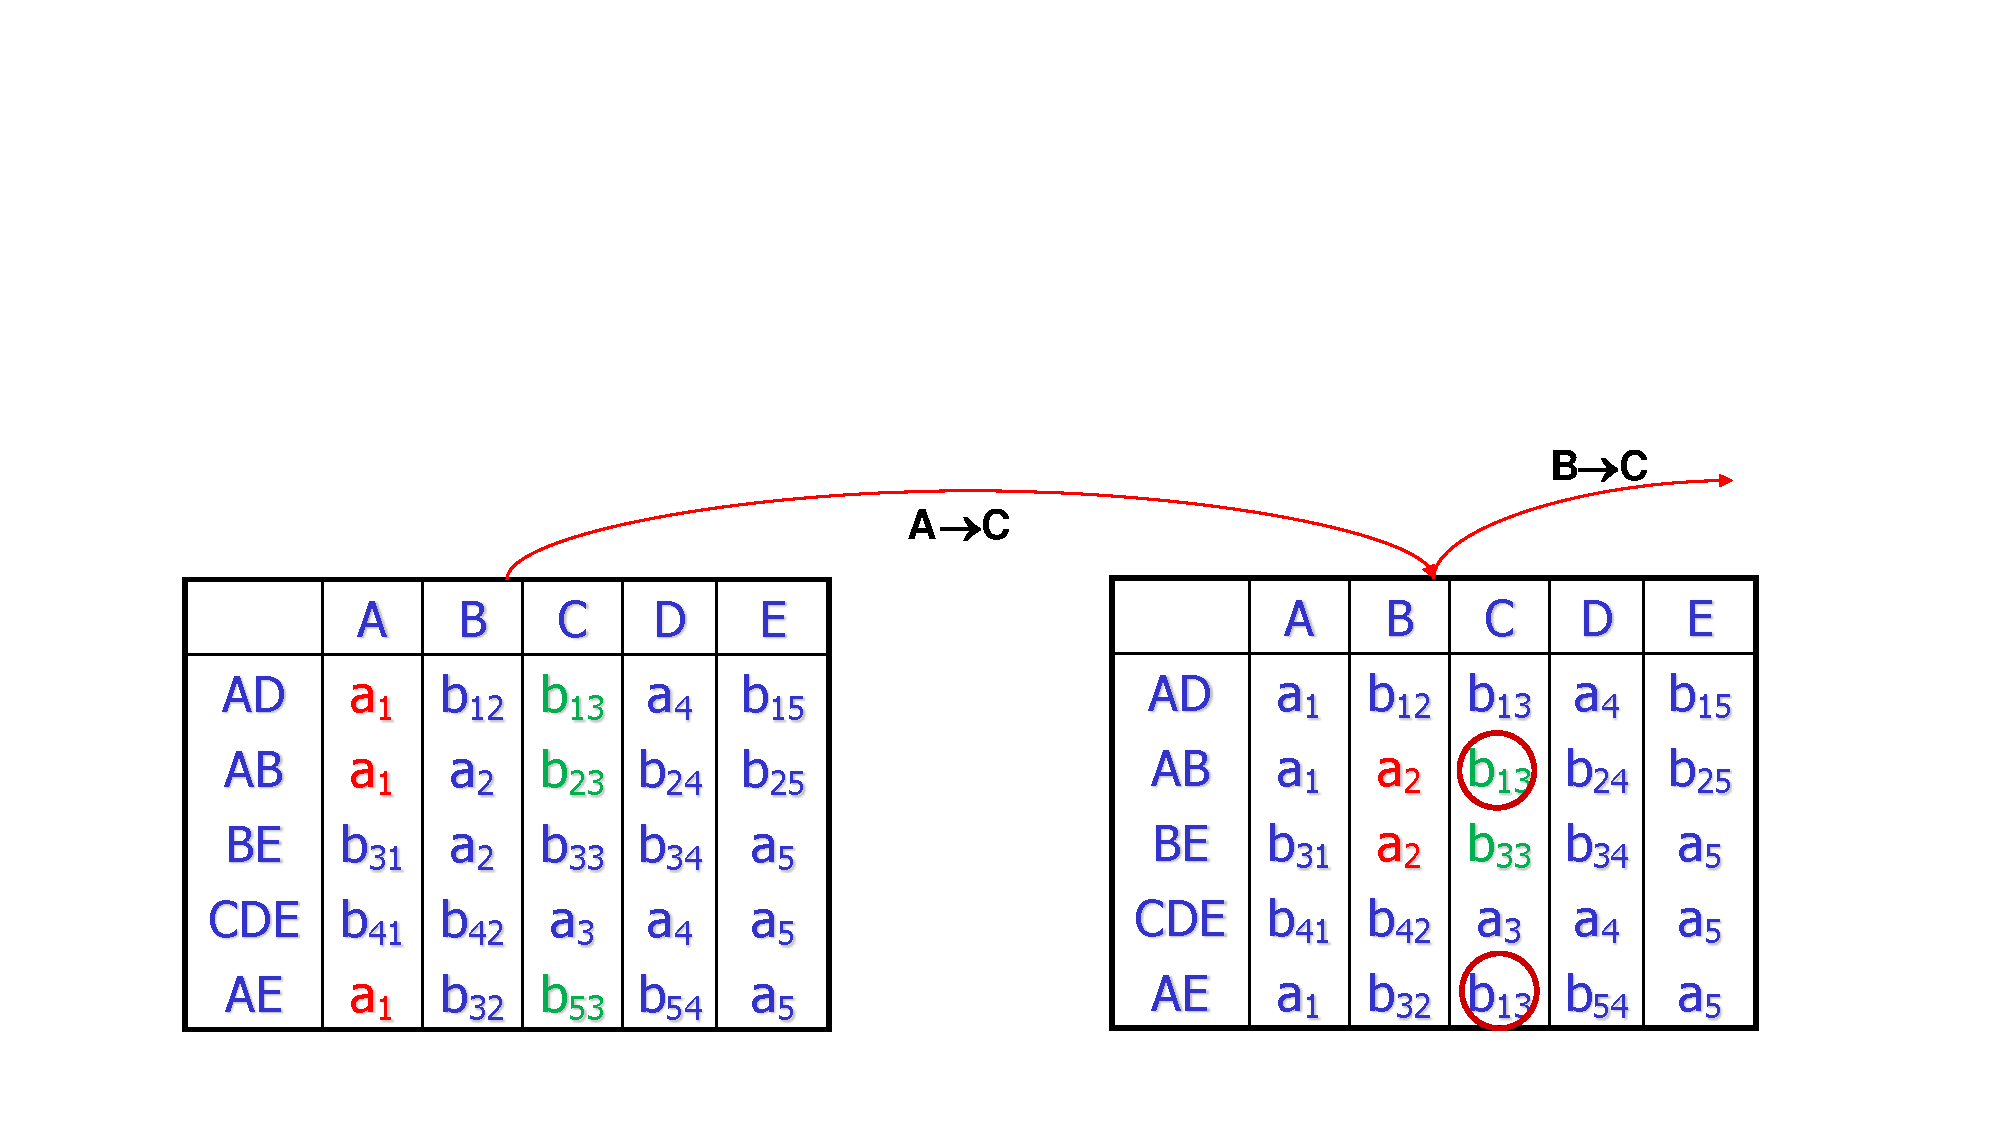
\includegraphics[width=.45\textwidth]{./figure/1.pdf}
    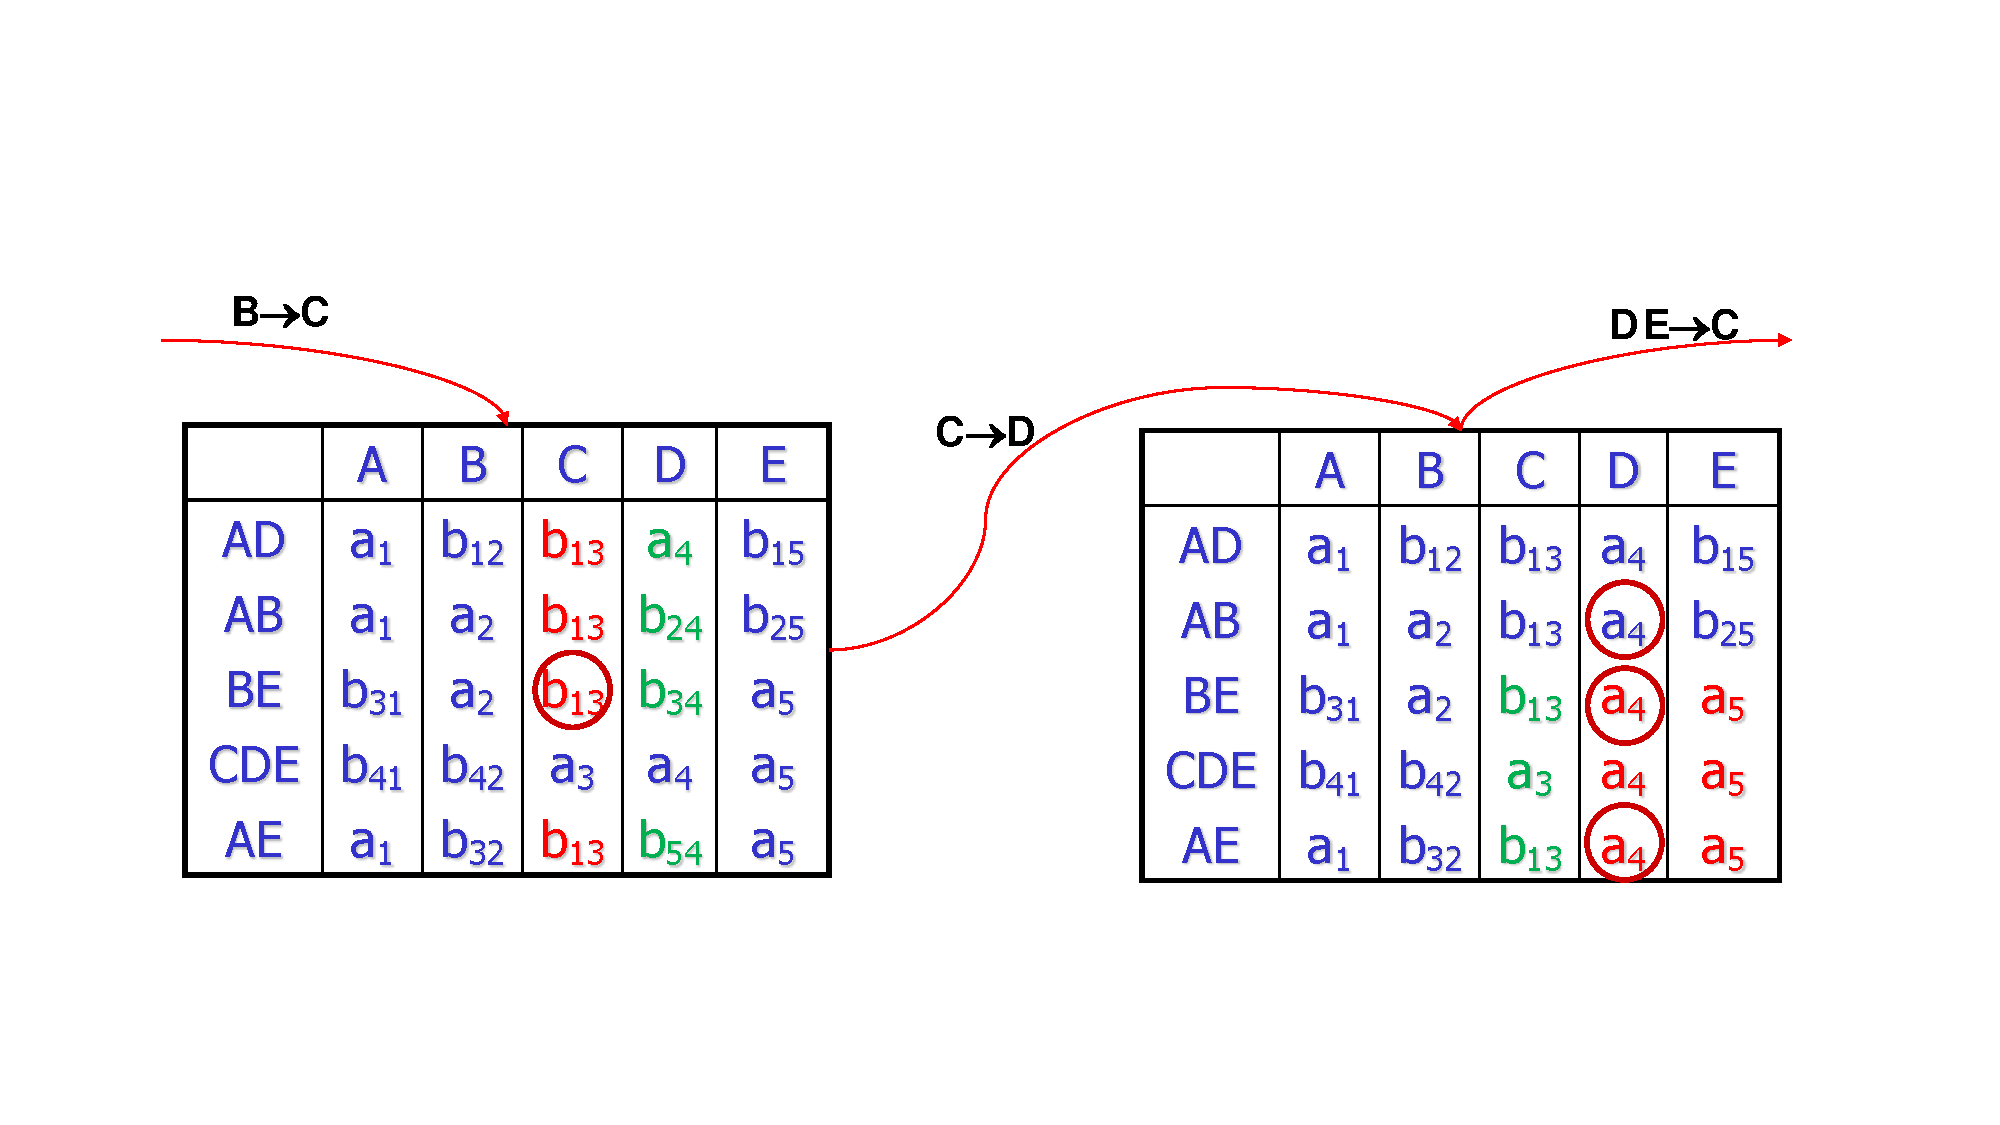
\includegraphics[width=.45\textwidth]{./figure/2.pdf}
    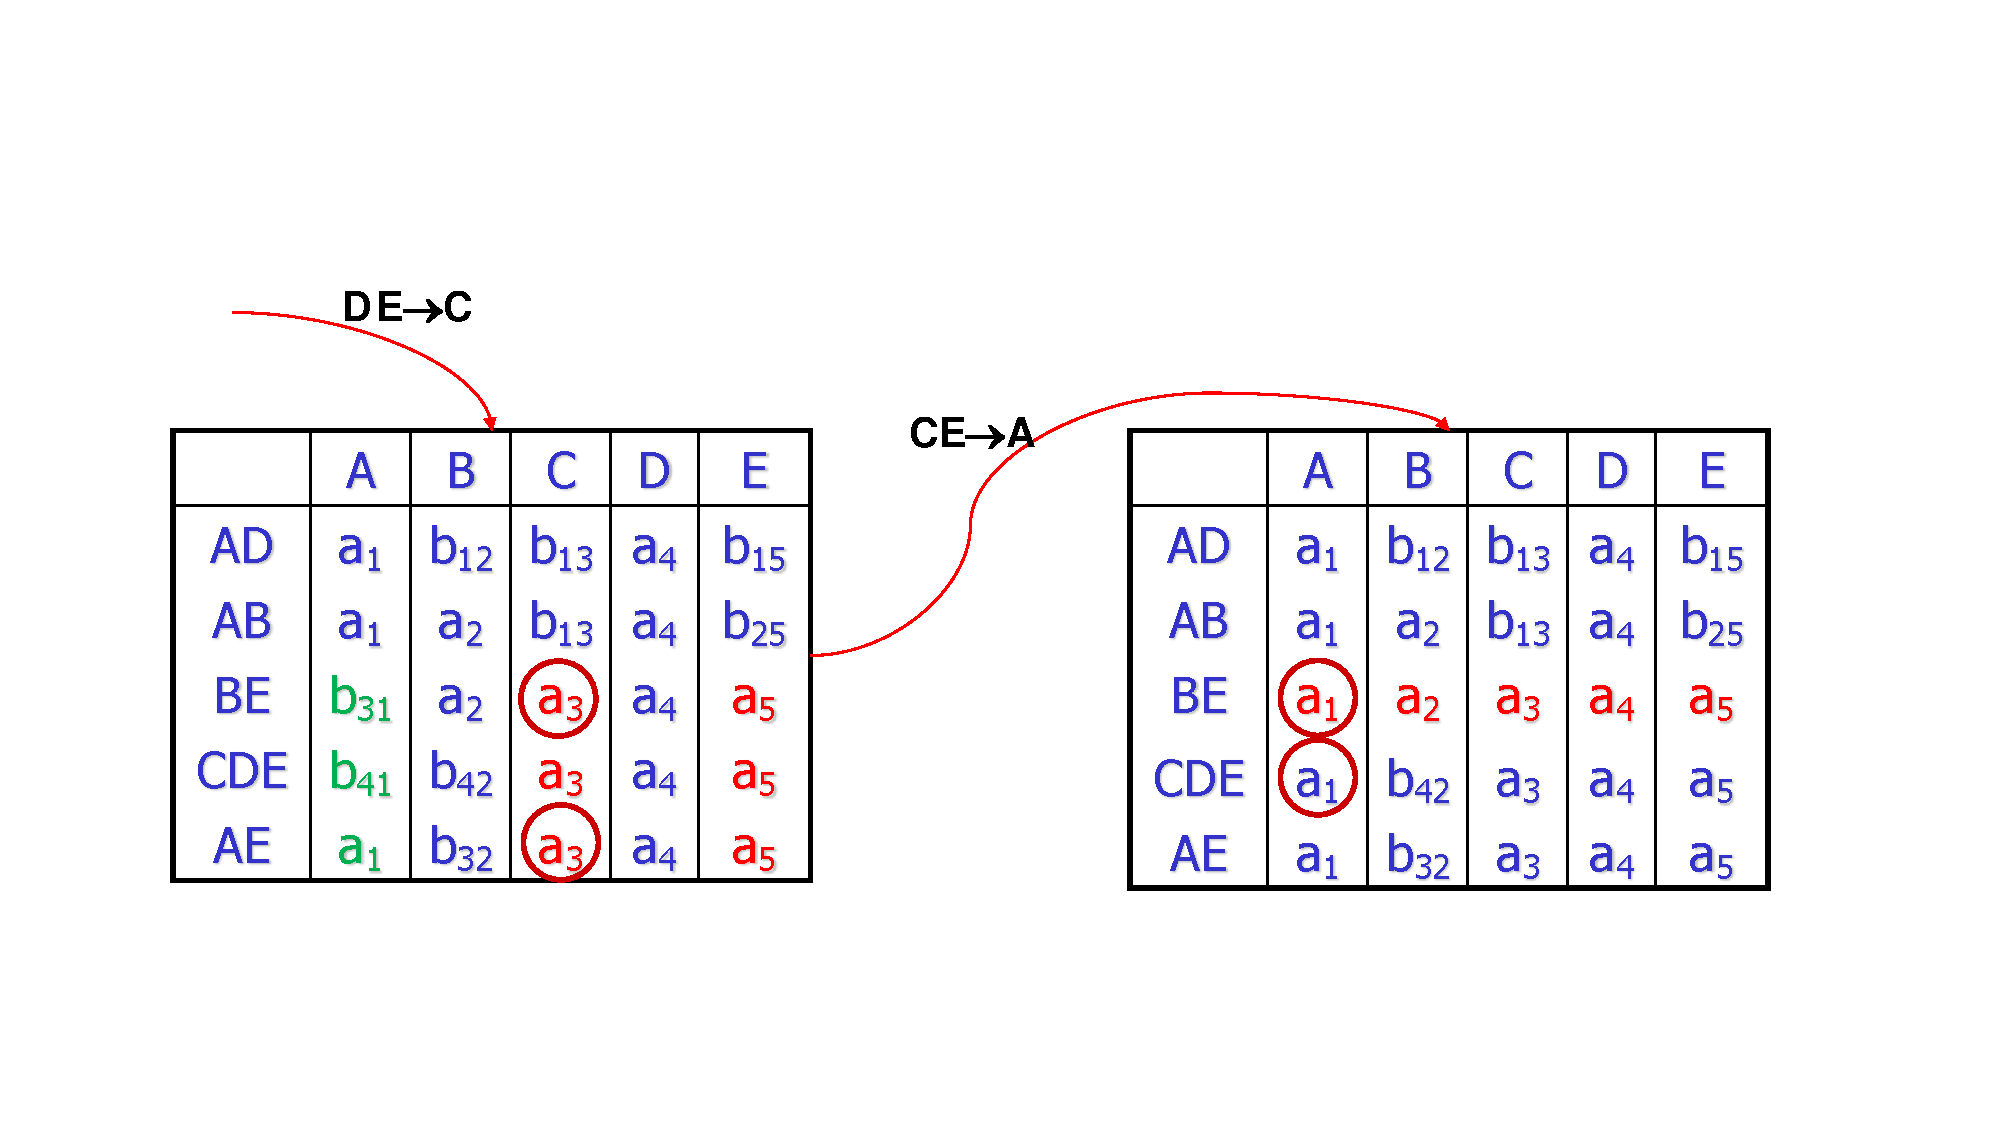
\includegraphics[width=.5\textwidth]{./figure/3.pdf}
    \caption{无损连接分解判别算法示例}
\end{figure}

分解为两个关系模式的无损分解判定算法:

$\rho=\{U_1,U_2\}$是无损连接分解 $\Leftrightarrow$ \textcolor{red}{$U_1\cap U_2\to U_1-U_2$ 或者 $U_1\cap U_2 \to U_2-U_1$}.


\subsection{关系模式分解算法}

\subsubsection{达到BCNF无损连接分解算法}

给定关系模式$R(U,F)$
\begin{enumerate}
    \item 令$\rho=R(U,F)$;
    \item 检查$\rho$中各关系模式是否属于BCNF, 若是, 则算法终止;
    \item 设$\rho$中$R_i(U_i,F_i)$不属于BCNF.

    则存在函数依赖\textcolor{red}{$X\to A\in F_i^+$, 且$X$不是$R_i$的码.}

    我们将$R_i$分解为$\sigma= \{S_1(U_1), S_2(U_2)\}$, 其中\textcolor{red}{$U_1=XA$, $U_2=U_i-A$}, 我们以$\sigma$代替$R_i$, 返回到2.
\end{enumerate}

\begin{theorem}
  上述算法得到的分解是无损连接分解.
\end{theorem}

\begin{proof}
  上述算法中出现的分解操作在第3步, 只要证明这个分解是无损连接分解, 那么整个算法得到的分解都是无损连接分解.

  根据判断分解为两个关系模式的无损分解判定方法, 我们发现: $U_1\cap U_2=X$, $U_1-U_2=A$, 而已知$X\to A$, 那么就有$U_1\cap U_2\to U_1-U_2$, 从而是无损连接分解.

  那么上述算法得到的是无损连接分解.
\end{proof}

\begin{theorem}
  上述算法分解得到的每个关系模式都是BCNF的.
\end{theorem}

\begin{proof}
  因为每次都会进行一次分解, 那么至多进行$|F^+|$次分解, 最后得到的一定是BCNF.
\end{proof}


\begin{example}
  $ U = \{A, B, C, D, E\}, F = \{A \rightarrow B, B \rightarrow C, AD \rightarrow E\}$.
\end{example}

码是\textcolor{red}{$AD$}, \textcolor{teal}{$A\to B$, $B\to C$}违反了BCNF.

\begin{figure}[H]
    \centering
    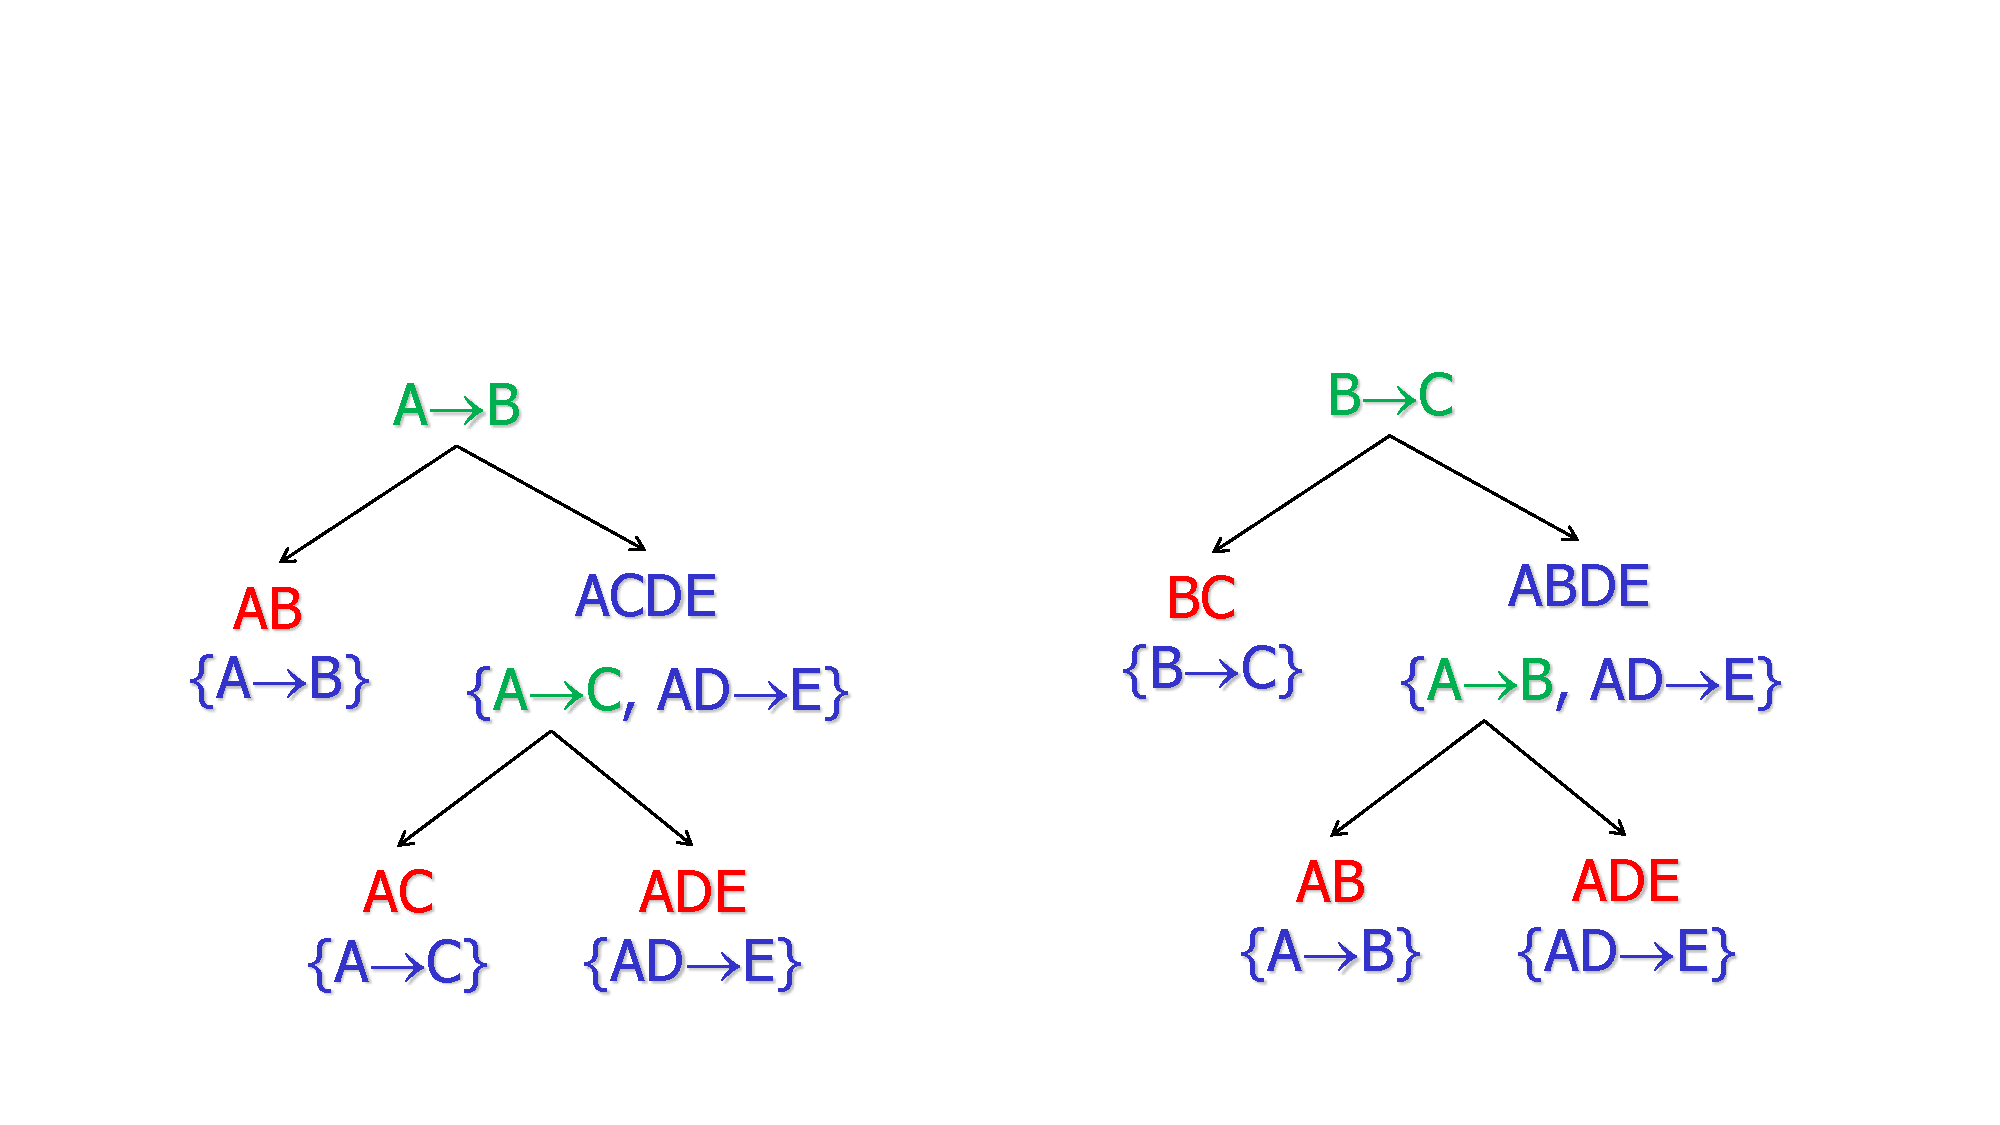
\includegraphics[width=.8\textwidth]{./figure/BCNF无损分解.pdf}
    \caption{达到BCNF无损连接分解算法}
\end{figure}

\begin{example}
  如何构造一个有$N$种BCNF分解结果的关系模式?
\end{example}

$R(A_0A_1\dots A_n; \{A_0\to A_n, A_1\to A_n, A_2\to A_n, \dots, A_{n-1}\to A_n\})$.

\begin{example}
  $R(A_1A_2\dots A_n; \{A_1\to A_2, A_2\to A_3, \dots, A_{n-1}\to A_n\})$有多少种BCNF分解结果?
\end{example}

\textcolor{red}{可以把BCNF分解算法改进为: 使用$X^+$.}

\textcolor{red}{若要求分解保持函数依赖, 那么分解后的模式总可以达到3NF, 但不一定能达到BCNF.}

\subsubsection{达到4NF无损连接分解算法}

给定关系模式$R(U,F)$,
\begin{enumerate}
    \item 令$\rho = R(U,F)$;
    \item 检查$\rho$中各关系模式是否属于4NF, 若是, 则算法终止;
    \item 设$\rho$中$R_i(U_i,F_i)$不属于4NF,

        存在非平凡多值依赖\textcolor{red}{$X \rightarrow \rightarrow A$}, 且\textcolor{red}{$X$}不是\textcolor{red}{$R_i$}的码,

        将$R_i$分解为$\sigma = \{S_1(U_1), S_2(U_2)\}$,
        其中$U_1 = XA$, $U_2 = U_i - A$,

        以$\sigma$代替$R_i$, 返回到 2.
\end{enumerate}

\begin{example}
  $U=\{A,B,C,D,E,G\}, F=\{A\to\to BCG, B\to AC, C\to G\}$, 码为$BDE$.
\end{example}

\begin{figure}[H]
    \centering
    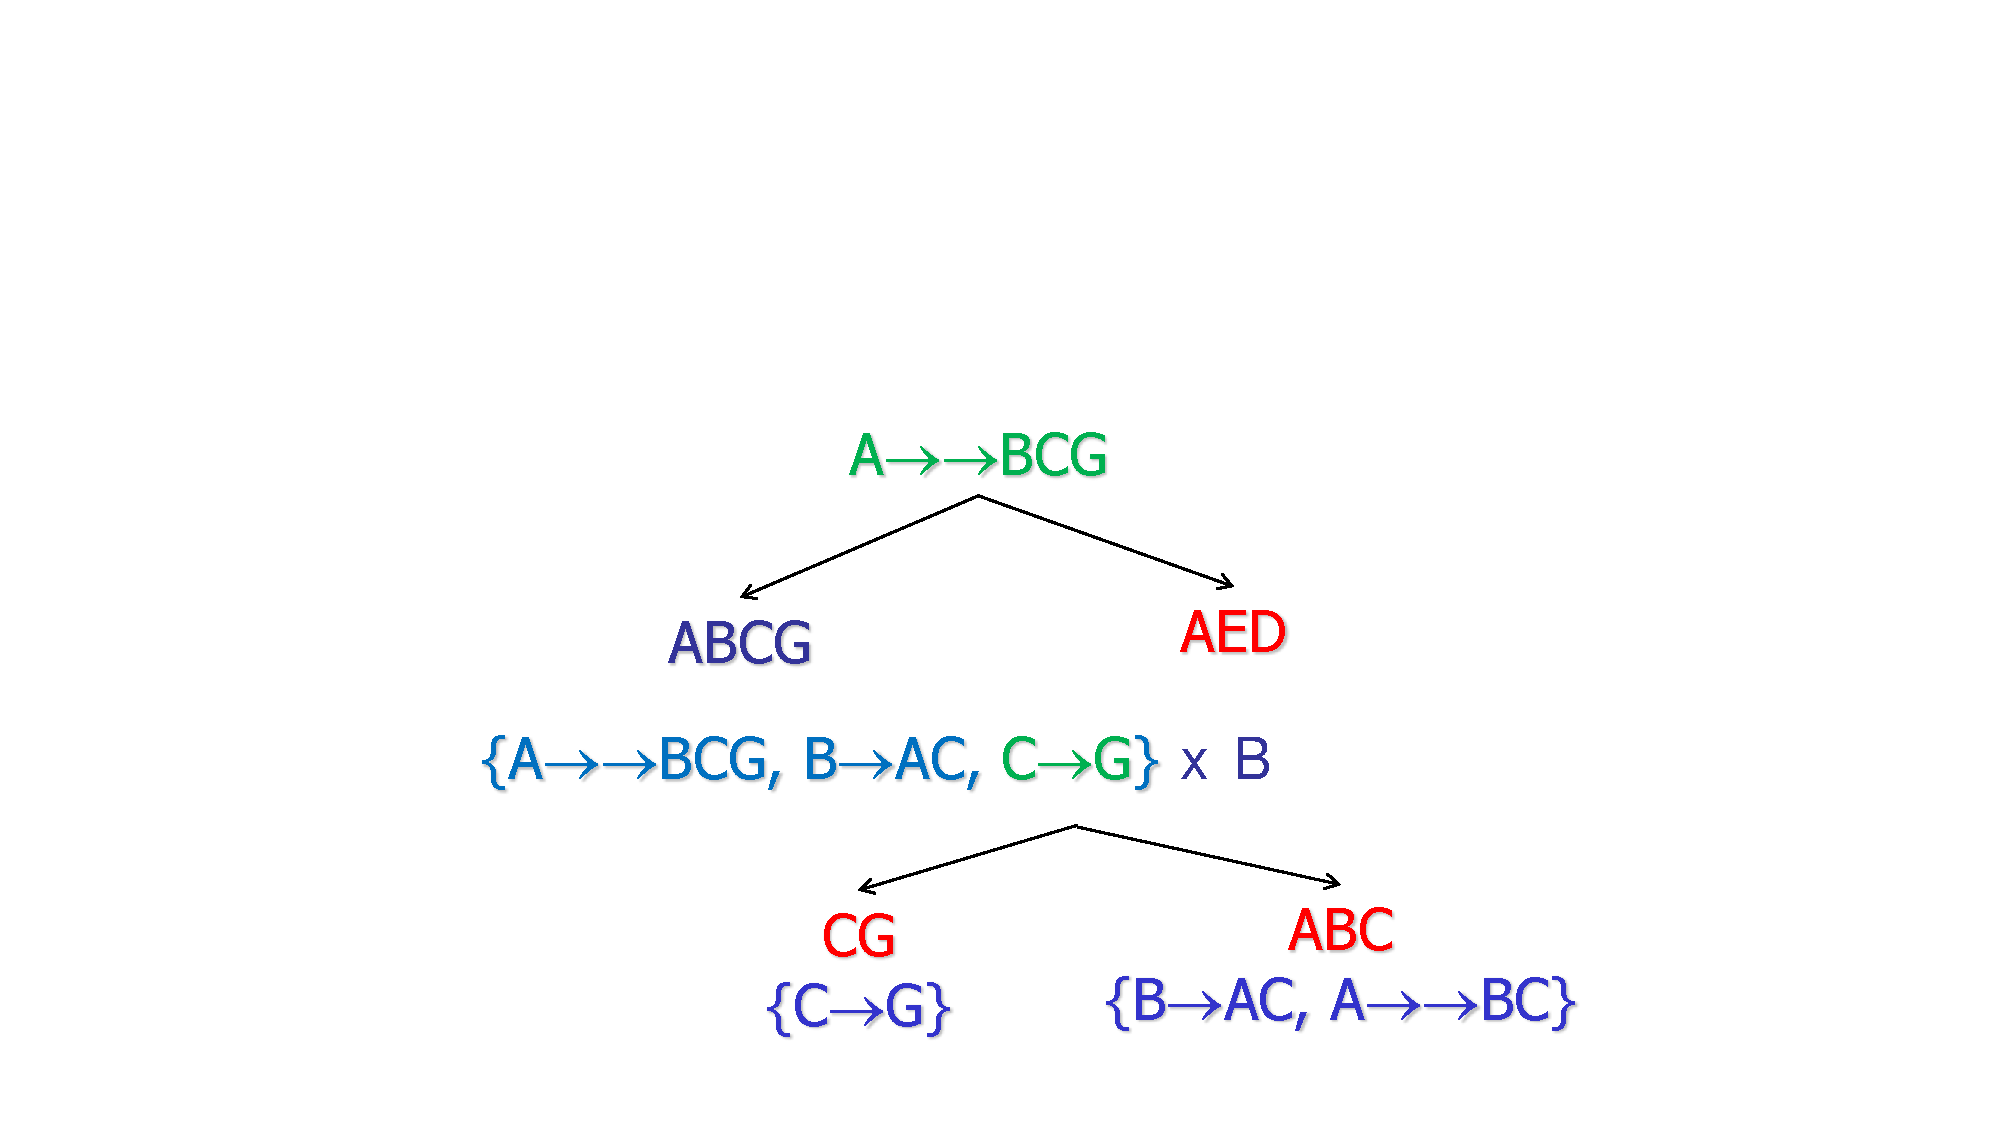
\includegraphics[width=.6\textwidth]{./figure/4NF无损连接分解.pdf}
    \caption{达到4NF无损连接分解算法}
\end{figure}

\subsubsection{达到3NF保持函数依赖的分解}

\begin{enumerate}
    \item 求$F$的最小覆盖$F_{min}$;
    
    \item 找出不在$F_{min}$中出现的属性, 将它们构成一个关系模式, 并从$U$中去掉它们(剩余属性仍记为$U$);
    
    \item 若有$X \rightarrow A \in F_{min}$, 且$XA = U$, $\rho = \{R\}$, 算法终止;
    
    \item 对$F_{min}$按具有相同左部的原则进行分组(设为$k$组),每一组函数依赖所涉及的属性全体为$U_i$, 令$F_i$为$F_{min}$在$U_i$上的投影, 则$\rho = \{R_1(U_1,F_1), R_2(U_2,F_2), ..., R_k(U_k,F_k)\}$是$R(U,F)$的一个保持函数依赖的分解, 并且每个$R_i(U_i,F_i) \in \text{3NF}$.
\end{enumerate}

>> 3NF分解算法的第3步, 如何确定此时关系模式已经是3NF的了?

>> 此时第2步去掉的属性不依赖留下的属性, 互相也不依赖, 必然是3NF的. 
而且第3步$X\to A\in F_{min}$, 而$F_{min}$中的依赖是单属性化和无冗余化的, 
从而属性$A$不可能传递依赖于$X$(否则就会违反了无冗余的性质), 同时$X$中的属性都是主属性, 所以这时关系模式已经是3NF的了.

\subsubsection{同时保持函数依赖和无损连接的分解算法}

设$\rho = \{ R_1(U_1,F_1), R_2(U_2,F_2), ..., R_k(U_k,F_k) \}$是$R(U,F)$的一个保持函数依赖的3NF分解, 设\textcolor{red}{$X$}是$R(U,F)$的码.

设若有某个$U_i$, \textcolor{red}{$X \subseteq U_i$}, 则$\rho$即为所求;
否则令$\tau = \rho \cup \{ R^*(X,F_X) \}$, \textcolor{red}{$\tau$}即为所求.

% TODO! why?

\begin{definition}[悬挂元组]
  $R$分解为$R_1,R_2,...,R_n$, \textcolor{red}{$r_1\bowtie r_2\bowtie \cdots \bowtie r_n$}称为\textcolor{red}{泛关系}.

  在$r_i$中出现, 但是在$\Pi_{R_i}(r_1\bowtie r_2\bowtie \cdots \bowtie r_n)$中没有出现的元组, 称为\textcolor{red}{悬挂元组}.
\end{definition}

悬挂元组代表了不完整的信息.
\begin{figure}[H]
    \centering
    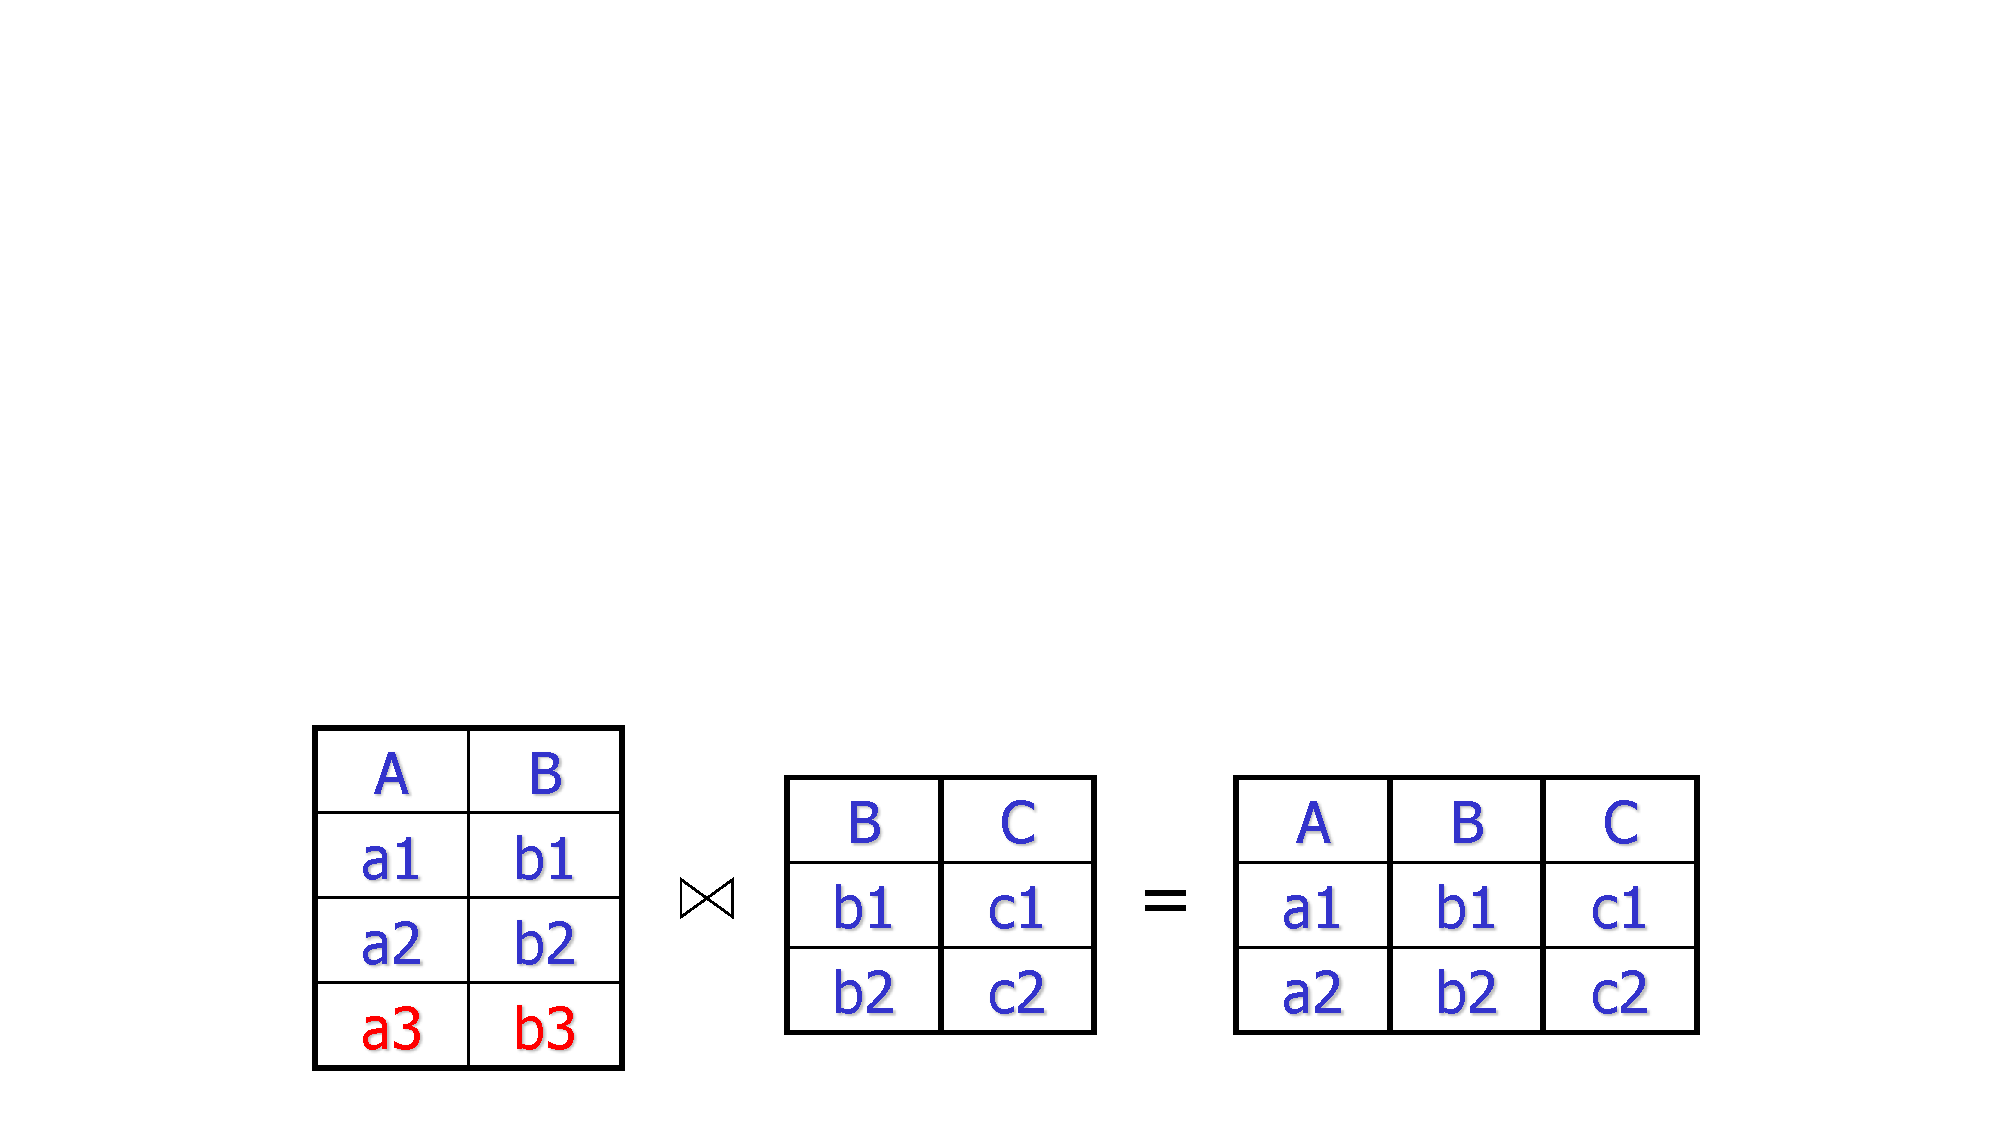
\includegraphics[width=.6\textwidth]{./figure/悬挂元组.pdf}
    \caption{悬挂元组}
\end{figure}

\section{模式调优}

\begin{itemize}
  \item 分解通常使得对复杂查询的回答的效率更差, 因为在查询求值期间必须执行额外的连接.
  \item 分解使得对简单查询的回答更有效, 因为这种查询通常涉及相同关系的一小部分属性.
  \item 分解通常使得简单的更新事务更有效.
  \item 分解能降低存储空间的要求, 因为它一般能消除冗余数据.
  \item 如果冗余级别低, 则分解会增加存储的需求.
\end{itemize}

\subsection{垂直划分}

$R(XYZ)$还是$R_1(XY)$和$R_2(XZ)$?

>> 一般情况下$R$好于$R_1$和$R_2$, 但是下面的情况除外:
\begin{enumerate}
    \item 大多数用户的存取分别在两个集合上;
    \item 属性$Y$和$Z$的值占用很大空间.
\end{enumerate}

事务-属性交叉矩阵(Transaction-Attribute Cross Matrix)是数据库物理设计与数据挖掘中, 
用于表示“哪个事务访问了哪些属性”的一种二元(0/1)矩阵结构. 
该矩阵的行对应系统中的各个事务(Transaction), 
列对应数据的各个属性(Attribute), 矩阵元素若为1, 则表示该事务访问(读或写)了该属性, 否则为0. 
通过对该矩阵进行聚类或分区, 可以识别在同一事务集中频繁共同访问的属性, 
从而指导垂直分区或矩阵聚类, 优化磁盘I/O与事务并发性能.

属性关联矩阵 $\to$ 属性带权关联图 $\to$ 图分割.
